%% ============================================================================
%% TDDMachine manuscript — unofficial Enfoque UTE template (IEEE format, 2026).
%% English body with a Spanish abstract (resumen), as required by the journal.
%%
%% Compilation (Windows, MiKTeX/TeX Live):
%%   pdflatex main_EN.tex
%%   bibtex   main_EN
%%   pdflatex main_EN.tex
%%   pdflatex main_EN.tex
%% ============================================================================

\documentclass[10pt,journal,twoside,letterpaper]{IEEEtran}

%% ============================================================================
%% >>>>>>>>>>>>>>>>>>>>>  FIELDS TO COMPLETE BEFORE SUBMISSION  <<<<<<<<<<<<<<<<<
%% Replace the TEXT INSIDE THE BRACES of each macro with the real value. Do not
%% change anything else: these values are inserted automatically into the body
%% of the article (Methodology and the code-availability statement).
%% ----------------------------------------------------------------------------
\newcommand{\llmversion}{claude-3-5-sonnet-XX}          % <-- exact model version, e.g.: claude-3-5-sonnet-20241022
\newcommand{\llmtemperatura}{YY}                        % <-- temperature used, e.g.: 0.2
\newcommand{\llmmaxtokens}{ZZ}                          % <-- output-token limit, e.g.: 4096
\newcommand{\llmperiodo}{WW}                            % <-- API access period, e.g.: March--April 2025
\newcommand{\repourl}{https://github.com/USER/tddmachine}  % <-- real public repository URL
%% ============================================================================

%% ------------------ Encoding and languages ------------------
\usepackage[T1]{fontenc}
\usepackage[utf8]{inputenc}
%% Main language "english" (listed LAST): guarantees English structural IEEE
%% labels and stable PDF bookmarks (hyperref) with accented characters. The body
%% is composed in English; the Spanish resumen and palabras clave are provided
%% with the custom \resumen and \palabrasclave environments and are wrapped in a
%% Spanish language block so they hyphenate under Spanish rules.
\usepackage[spanish,english]{babel}
\shorthandoff{.<>}

%% ------------------ Geometry (US Letter, two-column IEEE style) -------
%% Balanced margins and a narrow column separation (0.25in) in the style of IEEE
%% Transactions, for wider columns and cleaner justification.
\usepackage[
letterpaper,
top=0.75in,
bottom=0.95in,
left=0.62in,
right=0.62in,
columnsep=0.25in,
headsep=12pt,
headheight=14pt,
footskip=28pt
]{geometry}

%% ------------------ Content packages ------------------
\usepackage{graphicx}
\usepackage{amsmath,amssymb,amsfonts}
\usepackage{array}
\usepackage{booktabs}
\usepackage{multirow}
\usepackage{textcomp}
\usepackage{xcolor}
\usepackage{url}
\usepackage[hidelinks]{hyperref}
\usepackage{cite}
\usepackage{orcidlink}
\usepackage[protrusion=true,expansion=true]{microtype} % cleaner justification

%% English structural labels (Enfoque UTE IEEE style). Applied at the start of
%% the document to override the babel-spanish definitions when the language is
%% temporarily switched for the resumen.
\AtBeginDocument{%
    \renewcommand{\abstractname}{Abstract}%
    \renewcommand{\figurename}{Fig.}%
    \renewcommand{\tablename}{TABLE}%
    \renewcommand{\refname}{References}%
    \renewcommand{\bibname}{References}%
}

%% ------------------ Figure and table settings ------------------
\graphicspath{{./figures/}{./}}
\renewcommand{\arraystretch}{1.2}

%% Place floats as close as possible to their first reference, respecting the
%% Enfoque UTE IEEE style (floats at the top/bottom of a column, never inline).
%% flafter prevents a float from appearing before it is cited; stfloats enables
%% bottom placement for double-column floats.
\usepackage{flafter}
\usepackage{stfloats}
\setcounter{topnumber}{4}
\setcounter{bottomnumber}{3}
\setcounter{totalnumber}{6}
\renewcommand{\topfraction}{0.95}
\renewcommand{\bottomfraction}{0.7}
\renewcommand{\textfraction}{0.06}
\renewcommand{\floatpagefraction}{0.72}
\renewcommand{\dbltopfraction}{0.95}
\renewcommand{\dblfloatpagefraction}{0.72}
\setlength{\floatsep}{8pt plus 2pt minus 4pt}
\setlength{\textfloatsep}{10pt plus 2pt minus 5pt}
\setlength{\dbltextfloatsep}{10pt plus 2pt minus 5pt}

%% ------------------ Institutional logo (first page) ------------------
\usepackage{fancyhdr}
%% The logo is placed in the header of the title page as a ZERO-HEIGHT box
%% (\smash), so it reserves no space and does not push the body down; the bottom
%% margin of the title page then matches the rest of the document.
\fancypagestyle{enfoqueutefirstpage}{%
    \fancyhf{}
    \renewcommand{\headrulewidth}{0pt}
    \renewcommand{\footrulewidth}{0pt}
    \fancyhead[C]{%
        \smash{\raisebox{-0.35in}{
\includegraphics[width=1.9in]{enfoque_ute_logo.png}}}%
    }
    \setlength{\headheight}{14pt}
}

%% ------------------ Spanish resumen and keyword blocks ------------------
\newenvironment{resumen}{%
    \vspace{0.3em}
    \noindent\normalfont\small\itshape\textbf{Resumen}\hspace{0.5em}\textmd{---}\hspace{0.3em}%
    \ignorespaces
}{%
    \par\vspace{0.3em}%
}
\newcommand{\palabrasclave}[1]{%
    \vspace{0.2em}
    \noindent\small\textit{Palabras Clave}~---~#1
    \par\vspace{0.4em}
}
\newcommand{\seccionfunding}[1]{%
    \vspace{0.6em}
    \noindent\textsc{Funding}
    \par\vspace{0.2em}
    \small #1
    \par
}
\newcommand{\seccionconflicto}[1]{%
    \vspace{0.6em}
    \noindent\textsc{Conflict of Interest}
    \par\vspace{0.2em}
    \small #1
    \par
}
\newcommand{\seccioniadeclaracion}[1]{%
    \vspace{0.6em}
    \noindent\textsc{Artificial Intelligence Statement}
    \par\vspace{0.2em}
    \small #1
    \par
}
\newcommand{\seccionetica}[1]{%
    \vspace{0.6em}
    \noindent\textsc{Ethics and Informed Consent}
    \par\vspace{0.2em}
    \small #1
    \par
}
\newcommand{\secciondatos}[1]{%
    \vspace{0.6em}
    \noindent\textsc{Data and Code Availability}
    \par\vspace{0.2em}
    \small #1
    \par
}

%% ============================================================================
%% ARTICLE METADATA
%% ============================================================================
\author{%
    Gleiston~Guerrero-Ulloa\textsuperscript{1,2}~\orcidlink{0000-0001-5990-2357},
    Kerly~M.~Triana-Arrieta\textsuperscript{1},
    Efraín~Díaz-Macías\textsuperscript{1}~\orcidlink{0000-0003-4087-029X},
    Carlos~Rodríguez-Domínguez\textsuperscript{2,3}~\orcidlink{0000-0001-5626-3115},
    and~Miguel~J.~Hornos\textsuperscript{2}~\orcidlink{0000-0001-5722-9816}%
    \thanks{\textsuperscript{1}School of Computer Science, Universidad Técnica Estatal de Quevedo (UTEQ), Quevedo 120501, Los Ríos, Ecuador. \textsuperscript{2}Department of Software Engineering, University of Granada, 18071 Granada, Spain. \textsuperscript{3}Research Centre for Information and Communication Technologies (CITIC), University of Granada, 18071 Granada, Spain.}%
    \thanks{\emph{Corresponding author:} C. Rodríguez-Domínguez (e-mail: carlosrodriguez@ugr.es).}%
}

\markboth{Enfoque UTE (manuscript under review), 2026}%
{Guerrero-Ulloa \MakeLowercase{\textit{et~al.}}: LLM-Based Generation of the Initial TDD Test State}

%% ============================================================================
%% ARTICLE BODY
%% ============================================================================
\begin{document}
    
    \IEEEoverridecommandlockouts
    \pretolerance=10000
    
    \title{TDDMachine: Automatic Generation of the Initial Test State for Test-Driven Development Using a Large Language Model}
    
    \maketitle
    \thispagestyle{enfoqueutefirstpage}
    
    \begin{abstract}
        Writing test cases by hand is still a laborious, repetitive, and error-prone activity, and empirical evidence shows that developers test far less than they believe, treating testing as a low-value chore. Test-Driven Development (TDD), in which tests are written before production code, is nevertheless associated with 40--90\% lower defect density at the cost of only a modest increase in initial development effort. This paper presents TDDMachine, a Computer-Aided Software Engineering (CASE) tool that automates the generation of the initial test state---the \emph{Red} stage of the TDD cycle---from structured specifications (functional requirements, use cases, and user stories) using the Claude 3.5 Sonnet large language model (LLM). The requirements were derived from a systematic literature review of 109 primary studies; the technology stack (React~18, Django~4.2, PostgreSQL~15, Docker) was chosen through a weighted multi-criteria evaluation; and the generated \texttt{pytest} scripts are syntactically validated through Python abstract syntax tree analysis. The tool was evaluated with 25~participants using the System Usability Scale (SUS) and the Technology Acceptance Model (TAM), and with 10~experts who assessed test quality through a structured rubric. TDDMachine produced valid scripts in 91.4\% of attempts, reached a mean expert-rated quality of 4.08/5.0, obtained a SUS score of 74.46/100 (``Good''), and exceeded the technology-acceptance threshold across all four TAM constructs. The results give empirical evidence that structured, LLM-assisted generation of the initial TDD state is both feasible and well accepted.
    \end{abstract}
    
    \begin{IEEEkeywords}
        CASE tool; automated test generation; generative artificial intelligence; large language models; Test-Driven Development; pytest; software quality assurance; requirements engineering.
    \end{IEEEkeywords}
    
    \begin{otherlanguage}{spanish}
        \begin{resumen}
            La creación manual de casos de prueba sigue siendo una tarea laboriosa, repetitiva y propensa a errores, y la evidencia empírica muestra que los desarrolladores prueban mucho menos de lo que creen, percibiendo la escritura de pruebas como una carga de bajo valor; sin embargo, el Desarrollo Guiado por Pruebas (TDD), en el que las pruebas se escriben antes que el código de producción, se asocia con una reducción de la densidad de defectos del 40--90\,\% a cambio de un incremento moderado del esfuerzo inicial. Este artículo presenta TDDMachine, una herramienta CASE que automatiza la generación del estado inicial de las pruebas (la etapa \emph{Red} del ciclo TDD) a partir de especificaciones estructuradas (requisitos funcionales, casos de uso e historias de usuario) mediante el modelo de lenguaje de gran escala (LLM) Claude 3.5 Sonnet. Los requisitos se derivaron de una revisión sistemática de 109 estudios primarios; la pila tecnológica (React~18, Django~4.2, PostgreSQL~15, Docker) se seleccionó mediante evaluación multicriterio ponderada; y los scripts \texttt{pytest} generados se validan sintácticamente mediante análisis del árbol sintáctico abstracto de Python. La herramienta se evaluó con 25 participantes mediante los instrumentos SUS y TAM, y con 10 expertos que valoraron la calidad de las pruebas mediante una rúbrica estructurada. TDDMachine produjo scripts válidos en el 91,4\,\% de los intentos, alcanzó una calidad media evaluada por expertos de 4,08/5,0, obtuvo un puntaje SUS de 74,46/100 (``Bueno'') y superó el umbral de aceptación tecnológica en los cuatro constructos TAM. Los resultados aportan evidencia empírica de que la generación estructurada del estado inicial TDD asistida por LLM es viable y bien aceptada.
        \end{resumen}
        
        \palabrasclave{herramienta CASE; generación automática de pruebas; inteligencia artificial generativa; modelos de lenguaje de gran escala; Desarrollo Guiado por Pruebas; pytest; aseguramiento de calidad; ingeniería de requisitos.}
    \end{otherlanguage}
    
    %% The body from here on uses English hyphenation. The IEEE labels are
    %% reasserted after the language switch so that "Fig." and "TABLE" prevail.
    \selectlanguage{english}
    \renewcommand{\figurename}{Fig.}
    \renewcommand{\tablename}{TABLE}
    \renewcommand{\refname}{References}
    \renewcommand{\bibname}{References}
    
    %% ------------------------------------------------------------------------
    \section{Introduction}
    \label{sec:introduccion}
    
    \IEEEPARstart{S}{oftware} testing is a cross-cutting activity of the development life cycle, responsible for verifying the functionality, stability, and reliability of code before it reaches production; yet writing tests by hand remains a costly and error-prone task, particularly in agile settings where delivery cycles are short and requirements change often \cite{lukasczyk2023empirical,wang2024survey}.
    
    This burden explains a well-documented tension in professional practice: although testing is recognized as essential, developers tend to regard it as a tedious activity of little immediate value, one that competes with writing features. Field studies bear this out. The study by Beller et~al., which instrumented the development environments of thousands of programmers, showed that developers spend far less time testing than they themselves estimate, and that a sizable share of development sessions goes by without a single test being run \cite{beller2015test}. In the same vein, the survey by Straubinger and Fraser reports that a significant proportion of developers find writing tests unappealing and routinely put it off in favor of other work \cite{straubinger2023survey}.
    
    Evidence on project outcomes, however, points the other way once tests are written ahead of code. Test-Driven Development (TDD) inverts the traditional coding order: first a test is written that fails because the code does not yet exist (the \emph{Red} stage), then the minimum code needed to make the test pass is implemented (the \emph{Green} stage), and finally the code is refactored while the tests stay green (the \emph{Refactor} stage) \cite{beck2003tdd}. The industrial study by Nagappan et~al., conducted across four teams at Microsoft and IBM, documented a drop in pre-release defect density of between 40\% and 90\% relative to comparable projects that did not apply TDD, at the cost of only a 15\% to 35\% increase in initial development time \cite{nagappan2008tdd}. The meta-analysis by Rafique and Mišić confirms a significant improvement in external quality associated with TDD, and the controlled experiment by Erdogmus et~al. on the \emph{test-first} approach found productivity gains attributable to writing tests first \cite{rafique2013meta,erdogmus2005testfirst}. Taken together, these results indicate that software built from its tests is more likely to deliver the committed functionality on schedule, and that the early maintenance phase---correcting defects found after delivery---tends to be smaller than when tests are written after the code.
    
    When in the life cycle the tests are written is therefore decisive. In the traditional \emph{test-last} approach, tests are written once the functionality has been implemented, so they act as after-the-fact verification and inherit the design decisions already made; in the \emph{test-first} approach that TDD promotes, by contrast, tests are written before the production code and operate as an executable specification that guides the design \cite{beck2003tdd,erdogmus2005testfirst}. Requirements engineering offers a natural starting point for this anticipation: when functional requirements, use cases, and user stories are documented in a structured way, following standards such as ISO/IEC/IEEE~29148, their acceptance criteria translate directly into verifiable test conditions \cite{iso29148}. The practical challenge is that writing those initial tests from requirements, and doing so before writing any code, demands a cognitive effort and a level of testing experience that many teams lack, which limits the adoption of TDD despite its demonstrated benefits \cite{ghafari2020inconclusive}.
    
    Faced with challenges of this kind, software engineering has begun to incorporate generative artificial intelligence (AI) to automate tasks that were traditionally manual. The most recent systematic reviews document that large language models (LLMs) are being applied, with measurable success metrics, across numerous processes of the life cycle---code generation and completion, program summarization and translation, defect repair, and requirements elicitation, among others---and not only in the testing phase \cite{hou2024llm4se,carleton2024genai}. This trend is also reflected in regional research output: \emph{Enfoque UTE} has published reviews and studies reporting the application of machine learning and deep learning to engineering problems with quantitative performance indicators, from classification with artificial neural networks \cite{molina2024ann} to automatic bandwidth tuning in wireless networks \cite{carrillo2025ai} and the integration of the Internet of Things with artificial intelligence in agriculture \cite{basurto2026iotai}. In the specific field of testing, LLMs have shown the ability to interpret natural-language specifications and synthesize structured, executable test cases, with reported success rates that vary with the quality of the input specification \cite{wang2024survey,yang2024evaluation,rehan2025harnessing,bhatia2024unit,korraprolu2025testcase,takerngsaksiri2025pytester}.
    
    AI-based tools for test generation nonetheless have strengths and limitations that are worth contrasting with the proposal of this work. \emph{ChatUniTest} \cite{chen2024chatunitest}, \emph{TestSpark} \cite{sapozhnikov2024testspark}, and \emph{Pynguin} \cite{lukasczyk2022pynguin} generate unit tests effectively, but they do so from pre-existing source code, so they naturally operate in a \emph{test-last} scheme and integrate into the development environment; \emph{Pytester} \cite{takerngsaksiri2025pytester} does translate textual descriptions into test cases, though without structured requirements management or control of the cycle state. The strength of these tools is their maturity and coverage, and their main limitation, from a TDD standpoint, is that they presuppose the existence of the very code that the methodology proposes to write \emph{after} the test. The proposal of this work, TDDMachine, is deliberately positioned at an earlier phase of the cycle: it is a CASE (Computer-Aided Software Engineering) tool that acts exclusively on the \emph{Red}$\rightarrow$\emph{Green} transition of the TDD cycle, generating the Python test script with \texttt{pytest} from structured specifications, so as to hand the development team the starting point from which to write the minimal production code. The solution was developed by deriving its requirements from a systematic literature review, selecting its technology stack (React~18, Django~4.2, PostgreSQL~15, and container deployment with Docker) through a weighted multi-criteria evaluation, and integrating the Claude 3.5 Sonnet model through a structured prompt builder and a validator that checks the syntax of the generated code against Python's abstract syntax tree (AST). To assess the tool, two studies were designed in keeping with that scope: a usability and technology-acceptance study with 25 participants, using the SUS and TAM instruments, and a study of the quality of the generated tests with 10 experts, using a structured rubric.
    
    This work makes three contributions. First, TDDMachine, a CASE tool that integrates in a single workflow the structured capture of three types of specification (functional requirements, use cases, and user stories; FR, UC, and US), the generation of the initial test state with an LLM, and the syntactic validation of the generated code through Python's AST---a gap that none of the state-of-the-art tools covers in an integrated way. Second, a systematic review of 109 primary studies that characterizes the standards and notations used to structure requirements and their relationship with automatic test generation, and that grounds the design of the tool. Third, empirical evidence of the feasibility and acceptance of the proposal, obtained through a usability and technology-acceptance study with 25 participants and a test-quality study with 10 experts.
    
    The rest of the article is organized as follows. Section~\ref{sec:trabajos} presents a systematic literature review, conducted according to Kitchenham's guidelines, that positions the contribution against the state of the art. Section~\ref{sec:metodologia} describes the development and evaluation methodology. Section~\ref{sec:resultados} reports the generation, usability, acceptance, and quality results. Section~\ref{sec:discusion} discusses the findings against the objectives and prior work and sets out the threats to validity. Finally, Section~\ref{sec:conclusiones} summarizes the conclusions and lines of future work.
    
    %% ------------------------------------------------------------------------
    \section{Related Work}
    \label{sec:trabajos}
    
    To ground the requirements of TDDMachine and situate its contribution against the state of the art, we conducted a Systematic Literature Review (SLR) following the methodological guidelines of Kitchenham et~al., which structure the process into three phases---planning, execution, and reporting \cite{kitchenham2009slr}---and reported it in accordance with the 2020 PRISMA (Preferred Reporting Items for Systematic Reviews and Meta-Analyses) statement \cite{prisma2020}. Before execution, we defined a protocol fixing the research questions, the search strategy and strings, the inclusion and exclusion criteria (which incorporate the assessment of methodological quality as a criterion applied at full text, EC1), and the data-extraction procedure, so as to ensure the traceability and reproducibility of the review.
    
    \subsection{Research Questions}
    \label{subsec:rqs}
    
    The aim of the review is to determine how a software specification should be captured in a structured way to enable automatic test generation, a question that grounds the design of TDDMachine's input forms. From this aim, we derived the four research questions in Table~\ref{tab:rqs}: RQ1 asks about the existing standards for structuring requirements; RQ2, about the fields the capture forms should include; RQ3, about the way such structuring facilitates test generation; and RQ4, about the CASE tools that already implement these ideas and their limitations.
    
    \begin{table}[!tb]
        \caption{Research questions of the systematic review}
        \label{tab:rqs}
        \centering
        \small
        \begin{tabular}{@{}p{0.07\columnwidth}p{0.83\columnwidth}@{}}
            \toprule
            \textbf{ID} & \textbf{Research question} \\
            \midrule
            RQ1 & What standards and methodologies exist for the structured capture of functional requirements? \\
            RQ2 & What features should forms and schemas have in order to standardize the capture of specifications? \\
            RQ3 & How do these standards facilitate the automatic generation of test cases? \\
            RQ4 & What existing CASE tools implement these methodologies? \\
            \bottomrule
        \end{tabular}
    \end{table}
    
    \subsection{Search Strategy and Strings}
    \label{subsec:busqueda}
    
    The search strategy was structured with the PICOC framework (Population, Intervention, Comparison, Outcomes, Context), which operationalizes the aim of the review into five elements. Table~\ref{tab:picoc} details the terms assigned to each element.
    
    \begin{table}[!tb]
        \caption{Operationalizing the search with PICOC}
        \label{tab:picoc}
        \centering
        \small
        \begin{tabular}{@{}p{0.20\columnwidth}p{0.70\columnwidth}@{}}
            \toprule
            \textbf{Element} & \textbf{Terms} \\
            \midrule
            Population (P)   & Software systems, web applications, and software development projects. \\
            Intervention (I) & Requirements-capture standards, structured forms, documentation methodologies, and CASE tools. \\
            Comparison (C)   & Traditional versus structured approaches; different documentation standards. \\
            Outcomes (O)     & Specification standardization, ease of automatic test generation, and reduced documentation time. \\
            Context (C)      & Requirements engineering, software development, and automated testing. \\
            \bottomrule
        \end{tabular}
    \end{table}
    
    These five elements bound the population of interest (software projects and systems), the intervention (standards, forms, and tools for structured requirements capture), the comparison (structured versus traditional approaches), the expected outcomes (specification standardization and automatic test generation), and the context (requirements engineering and automated testing). From these terms, we built Boolean search strings specific to each type of specification---functional requirements, use cases, and user stories---which were applied over four databases (Scopus, IEEE~Xplore, ACM~Digital~Library, and Web of Science) and complemented with a search of open-source repositories (GitHub) to identify practical implementations. Table~\ref{tab:cadenas} presents those strings in canonical form.
    
    \begin{table*}[!tb]
        \caption{Search strings in canonical form (adapted to each database's syntax)}
        \label{tab:cadenas}
        \centering
        \footnotesize
        \begin{tabular}{@{}p{0.14\textwidth}p{0.80\textwidth}@{}}
            \toprule
            \textbf{Category} & \textbf{Search string} \\
            \midrule
            Functional requirements & \texttt{(\,"requirement* specification" OR "requirement* template" OR "requirement* boilerplate" OR "requirement* pattern" OR "structured requirement*" OR "controlled natural language"\,) AND (\,"requirements engineering" OR "software engineering"\,)} \\
            \addlinespace
            Use cases & \texttt{(\,"use case template" OR "use case specification" OR "use case model*" OR "use case description" OR "restricted use case" OR "structured use case"\,) AND (\,"requirements engineering" OR "software engineering"\,)} \\
            \addlinespace
            User stories & \texttt{(\,"user stor* template" OR "user stor* format" OR "user stor* pattern" OR "user stor* documentation" OR "structured user stor*"\,) AND (\,"acceptance criteria" OR "INVEST" OR "agile" OR "scrum" OR "requirements engineering"\,)} \\
            \bottomrule
        \end{tabular}
    \end{table*}
    
    As Table~\ref{tab:cadenas} shows, the strings use truncation (\texttt{*}) and idiomatic synonyms to maximize coverage, and they were adapted to the syntax of each database---Scopus (\texttt{TITLE-ABS-KEY}), Web of Science (\texttt{TS=}), IEEE~Xplore (\texttt{"All Metadata"}), and ACM~Digital~Library (\texttt{AllField})---while preserving the same conceptual blocks, so that retrieval was comparable across the four sources.
    
    \subsection{Selection Criteria and Screening Process}
    \label{subsec:seleccion}
    
    Study selection was governed by the inclusion criteria (IC) and exclusion criteria (EC) in Table~\ref{tab:criterios}, defined a priori and each assigned to a single stage of the process to prevent duplicate application, as indicated in the \emph{Stage} column of that table.
    
    \begin{table}[!tb]
        \caption{Inclusion and exclusion criteria applied}
        \label{tab:criterios}
        \centering
        \small
        \setlength{\tabcolsep}{4pt}
        \begin{tabular}{@{}l>{\raggedright\arraybackslash}p{0.60\columnwidth}l@{}}
            \toprule
            \multicolumn{2}{@{}l}{\textbf{Inclusion criteria (IC)}} & \textbf{Stage} \\
            \midrule
            IC1 & Published between 2015 and the search execution date. & Elig. \\
            IC2 & Describe standards, models, or methodologies for the structured capture of requirements. & Title/abs. \\
            IC3 & Present forms, schemas, or criteria to standardize specifications. & Title/abs. \\
            IC4 & Address the relationship between requirements structuring and test generation. & Title/abs. \\
            IC5 & Deal with CASE tools for requirements management. & Title/abs. \\
            IC6 & Published in English. & Elig. \\
            IC7 & Primary studies: journal articles, conference papers, book chapters, books, or doctoral theses. & Elig. \\
            \midrule
            \multicolumn{2}{@{}l}{\textbf{Exclusion criteria (EC)}} & \textbf{Stage} \\
            \midrule
            EC1 & Purely theoretical studies without practical application, or lacking sufficient empirical evidence, methodological rigor, or reporting clarity (insufficient quality). & Full text \\
            EC2 & Outside the thematic scope: do not address structured requirements capture or its relationship with test generation. & Title/abs. \\
            EC3 & Secondary studies (systematic reviews, surveys, and mappings) that provide no primary evidence. & Elig. \\
            EC4 & Non-articles (proceedings front matter, prefaces, and preliminary conference material) and gray literature without peer review (except official standards). & Elig. \\
            EC5 & Duplicates, preliminary versions, or overlaps between categories. & Dedup. \\
            EC6 & No access to the full text. & Full text \\
            \bottomrule
        \end{tabular}
        \\[3pt]
        {\footnotesize The \emph{Stage} column indicates the single PRISMA-flow filter (Fig.~\ref{fig:prisma}) at which each criterion is applied: Dedup.\ = deduplication; Elig.\ = eligibility (metadata: year, language, and document type); Title/abs.\ = title-and-abstract screening (thematic relevance); Full text = full-text reading (methodological quality).}
    \end{table}
    
    The process, illustrated in the PRISMA diagram of Fig.~\ref{fig:prisma}, comprises four consecutive filters. The first is the identification of the records retrieved by the strings of Table~\ref{tab:cadenas} in each database. The second removes duplicates (EC5), giving priority to the primary sources (ACM~Digital~Library and IEEE~Xplore) over the bibliographic indexes (Scopus and Web of Science), which replicate much of their content. The third is eligibility, in which all the formal criteria are applied at once, over the databases' metadata: publication year from 2015 (IC1), English language (IC6), and admissible document type---primary studies: journal articles, conference papers, book chapters, books, and doctoral theses (IC7)---while excluding non-articles---proceedings and preliminary conference material---(EC4) and secondary studies---reviews, surveys, and systematic mappings---(EC3). The fourth is title-and-abstract screening, which retains only the studies relevant to the operational aim of the review---that a structured requirements artifact be explicitly linked to the automatic generation or derivation of tests (IC2--IC5; EC2). In this way, document type is resolved once at eligibility, title-and-abstract screening is confined to thematic relevance, and the final stage---full-text reading---is reserved for the assessment of methodological quality (EC1) and the confirmation of access to the document (EC6).
    
    \begin{figure}[!tb]
        \centering
        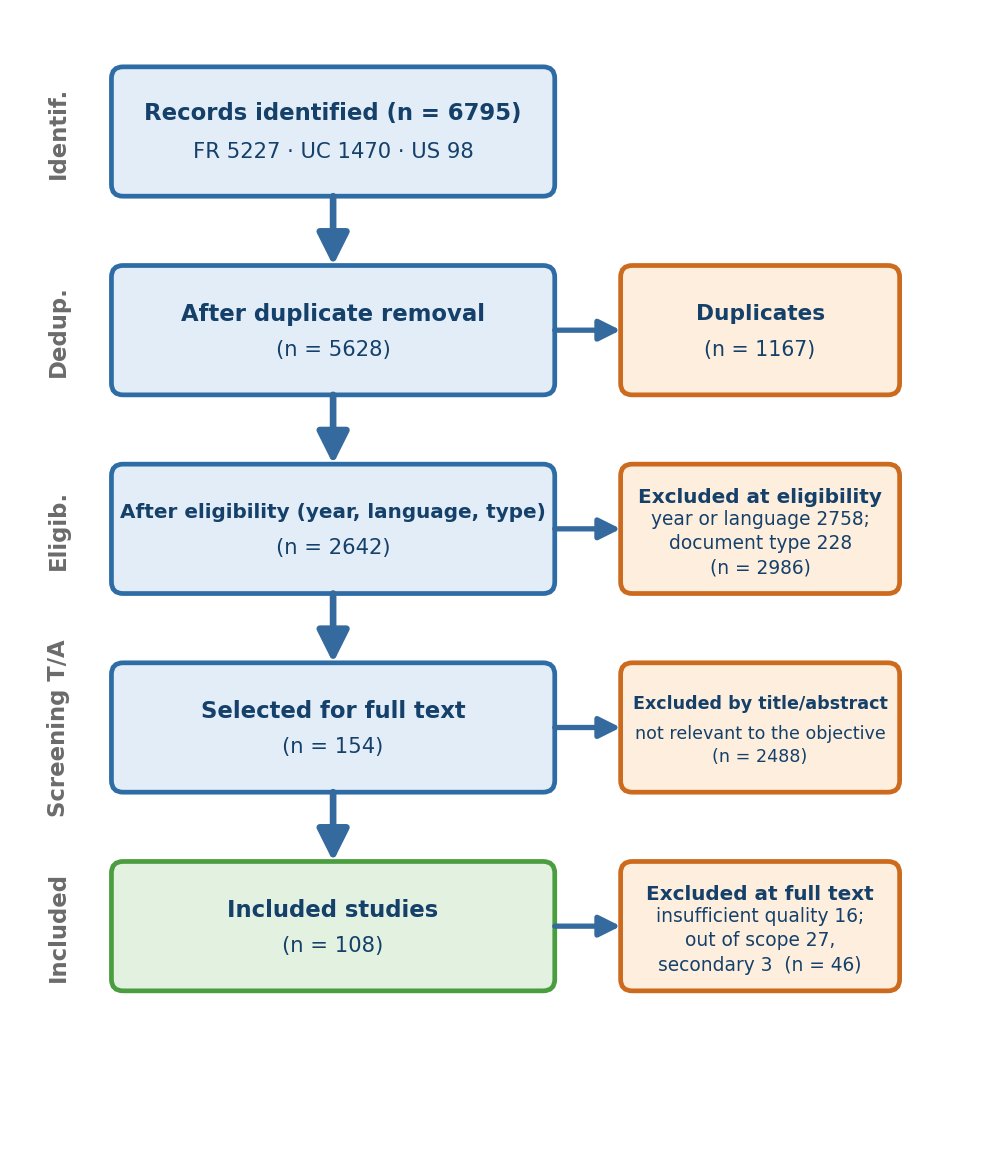
\includegraphics[width=\columnwidth]{fig_prisma.png}
        \caption{Consolidated PRISMA flow of the systematic review (functional requirements, use cases, and user stories across the four databases). Eligibility applies the criteria of year, language, and document type in a single stage; title-and-abstract screening is confined to thematic relevance; and of the 155 studies read at full text, 109 were included after assessing methodological quality.}
        \label{fig:prisma}
    \end{figure}
    
    Figure~\ref{fig:prisma} quantifies the outcome of each filter. Starting from 6,795 records identified in the four databases, the removal of duplicates---concentrated, as expected, in Scopus and Web of Science---leaves 5,628 unique records; the eligibility criteria---year, language, and document type---reduce them to 2,642 (2,758 records discarded by year or language and 228 by document type); and title-and-abstract screening---incorporating complementary studies for the user-story category, one study from the ICSR~2016 volume, and one functional-requirements study recovered after obtaining access to its full text---leaves 155 studies selected for full-text reading. These 155 were then read in full, a stage governed by the methodological-quality criterion (EC1): 109 studies were included and 46 were excluded---16 for insufficient methodological quality and 30 whose status as out of thematic scope (27) or as a secondary study (3) could only be confirmed with the full document. Table~\ref{tab:distrib} breaks down identification, deduplication, and eligibility by specification category and database.
    
    \begin{table*}[!tb]
        \caption{Identification, deduplication, and eligibility by specification category and database}
        \label{tab:distrib}
        \centering
        \small
        \setlength{\tabcolsep}{6pt}
        \begin{tabular}{@{}llccc@{}}
            \toprule
            \textbf{Specification} & \textbf{Database} & \textbf{Identified} & \textbf{After duplicates} & \textbf{After eligibility\textsuperscript{b}} \\
            \midrule
            \multirow{5}{*}{Functional requirements} & Scopus & 1,646 & 1,312 & 522 \\
            & Web of Science      & 1,607 & 1,066 & 379 \\
            & IEEE Xplore         & 961    & 947    & 409 \\
            & ACM Digital Library & 1,013\textsuperscript{a} & 1,013 & 859 \\
            \cmidrule(l){2-5}
            & \textbf{Subtotal}   & \textbf{5,227} & \textbf{4,338} & \textbf{2,169} \\
            \midrule
            \multirow{5}{*}{Use cases} & Scopus & 483 & 360 & 116 \\
            & Web of Science      & 310 & 173 & 55 \\
            & IEEE Xplore         & 138 & 136 & 49 \\
            & ACM Digital Library & 539 & 539 & 191 \\
            \cmidrule(l){2-5}
            & \textbf{Subtotal}   & \textbf{1,470} & \textbf{1,208} & \textbf{411} \\
            \midrule
            \multirow{5}{*}{User stories} & Scopus & 25 & 20 & 18 \\
            & Web of Science      & 18 & 7 & 4 \\
            & IEEE Xplore         & 6 & 6 & 4 \\
            & ACM Digital Library & 49 & 49 & 36 \\
            \cmidrule(l){2-5}
            & \textbf{Subtotal}   & \textbf{98} & \textbf{82} & \textbf{62} \\
            \midrule
            \textbf{Total} & & \textbf{6,795} & \textbf{5,628} & \textbf{2,642} \\
            \bottomrule
        \end{tabular}
        \\[3pt]
        {\footnotesize Duplicates were removed giving priority to the primary sources (ACM, IEEE) over the indexes (Scopus, Web of Science). \textsuperscript{a}\,The ACM export for functional requirements was limited to 2015--2026 (owing to the platform's export cap), so its \emph{Identified} column already excludes records before 2015. \textsuperscript{b}\,Eligibility: all formal criteria are applied to the metadata in a single stage---publication year $\geq$\,2015 (IC1), English language (IC6), and admissible document type: primary studies (journal articles, conference papers, book chapters, books, and doctoral theses; IC7), excluding non-articles (EC4) and secondary studies (EC3). Of the 5,628 unique records, 2,758 were discarded by year or language and 228 by document type; title-and-abstract screening (Table~\ref{tab:seleccion}) was applied to the 2,642 eligible records.}
    \end{table*}
    
    The breakdown in Table~\ref{tab:distrib} shows that functional requirements account for most of the retrieved records (5,227 of 6,795) and that the reduction by deduplication and eligibility is proportionally larger in Scopus and Web of Science, consistent with their role as indexes that largely replicate the output of the primary libraries. From the 2,642 eligible records, Table~\ref{tab:seleccion} reports, by category, how many studies were selected for full-text reading and how many were ultimately included.
    
    \begin{table}[!tb]
        \caption{Studies selected for full text and included, by category}
        \label{tab:seleccion}
        \centering
        \small
        \setlength{\tabcolsep}{6pt}
        \begin{tabular}{@{}lcc@{}}
            \toprule
            \textbf{Category} & \textbf{\shortstack{Selected for\\ full text\textsuperscript{a}}} & \textbf{Included\textsuperscript{b}} \\
            \midrule
            Functional requirements & 122 & 87 \\
            Use cases               & 22  & 13 \\
            User stories            & 11  & 9  \\
            \midrule
            \textbf{Total}          & \textbf{155} & \textbf{109} \\
            \bottomrule
        \end{tabular}
        \\[3pt]
        {\footnotesize \textsuperscript{a}\,Records passing title-and-abstract screening---confined to thematic relevance with the aim of the review (IC2--IC5; EC2)---starting from the 2,642 records already eligible by year, language, and document type; includes complementary studies for the user-story category, one study from the ICSR~2016 volume, and one functional-requirements study recovered after obtaining access to its full text. \textsuperscript{b}\,Studies that, after full-text reading, meet the sufficient methodological quality (EC1). Of the 155 read, 46 were excluded: 16 for insufficient methodological quality and 30 whose status as out of thematic scope (27) or as a secondary study (3) could only be confirmed with the full document.}
    \end{table}
    
    As Table~\ref{tab:seleccion} records, of the 155 studies read at full text, 109 were included, with inclusion rates of 71\% for functional requirements (87 of 122), 59\% for use cases (13 of 22), and 82\% for user stories (9 of 11); this last category, despite its smaller absolute volume, contributed the highest proportion of studies relevant to the aim of the review.
    
    \subsection{Data Extraction and Synthesis by Research Question}
    \label{subsec:sintesis}
    
    From each included study we extracted, using a standardized template, the following fields: year, authors, DOI, study type, application context, standards or methodologies described, specification fields identified, CASE tools mentioned, and relationship with automatic test generation. The full extraction of the 109 included studies---distributed as 87 on functional requirements, 13 on use cases, and 9 on user stories, and comprising 72 conference papers, 36 journal articles, and one doctoral thesis---is provided as supplementary material, and the set is referenced in full in \cite{Kudo2019Conceptual,Sandhu2026Framework,Bunder2019Model,Agrawal2023Requirements,Gupta2019Software,Mahanto2018Achieving,Kudo2023Aligning,Intana2023Approach,Intana2023Automated,Orekhov2026Example,Roldan2019Ontology,Trinh2026Fstg,Paiva2020Requirements,Oran2017Analysing,Veizaga2020Leveraging,Yue2015Rtcm,Wang2022Automatic,Zhang2018Specifying,Khamaiseh2017Software,Clerissi2017Towards,Li2026Test,Franca2026Req2test,Miranda2020Preliminary,Bhatia2025Automated,Jang2025Automatic,Longo2016Web,Tatale2020Enhancing,RochaSilva2020Ensuring,Gralha2021Impact,Araujo2017Generating,CorreaSouza2018Automated,Nogueira2016Automatic,Tiwari2015Approach,Wang2015Automatic,Baxter2023Roboworld,Carvalho2016Modelling,Ecar2018Cosmic,Saraiva2023Adoption,Matula2018Enterprise,Charoenreh2020Enhancing,Lim2024Test,Liu2022Ears2tf,Zheng2021Generating,Nguyen2023Analysis,Fischbach2019Automated,Olajubu2018Automated,Pudlitz2020What,Frattini2023Cira,HolodnikJanczura2017Extension,Lucassen2016Use,Abdeen2023Approach,Venkatesh2016Cost,Ansari2017Constructing,Wang2015Umtg,Erazo2017Maritaca,Louzaoui2016Invalid,Borg2022Quality,Wen2026Research,Liu2016Validating,Khaldi2026Agentic,Herwanto2025Enhancing,Wu2022Node,Martins2024Cm,Wiecher2019Test,Wiecher2021Besos,Wiecher2020Scenarios,Zafar2021Towards,Liu2022Automatic,Diniz2019Reducing,Shimizu2025Automatic,Salari2026Test,Wei2024Requirements,Palshikar2019Extraction,Saraiva2023Privacy,Rodriguez2023Behaviour,Medeiros2019Requirements,Fisher2016Making,Fathima2026Automated,Morales2024Dsl,Bandyszak2015Supporting,Silva2021Empirical,RochaSilva2022Towards,Arruda2026Deriving,LeonQuinstedt2026Rest,Jang2021Automatic,Hamza2020Generating,DosSantos2019Extraction,Fredericks2015Automated,Fazzolino2019Feature,Campanile2022Evaluation,Motwani2019Automatically,Moketar2016Testmereq,Jorge2018Integrating,Zafar2021Model,Varpe2025User,Sinha2015Requirements,Ishinari2025Improving,Ishinari2026Data,Chernorutsky2018Industrial,Mai2019Mcp,Trinh2026Tcg,Dilorenzo2026Recommending,Baker2026Industrial,Yue2016Practical,Tran2025Famres,DosSantos2018Automated,Malik2020Automating,Osama2021Srcm,Crapo2017Requirements}; Fig.~\ref{fig:years} presents the temporal distribution of this set by requirements-artifact category.
    
    \begin{figure}[!tb]
        \centering
        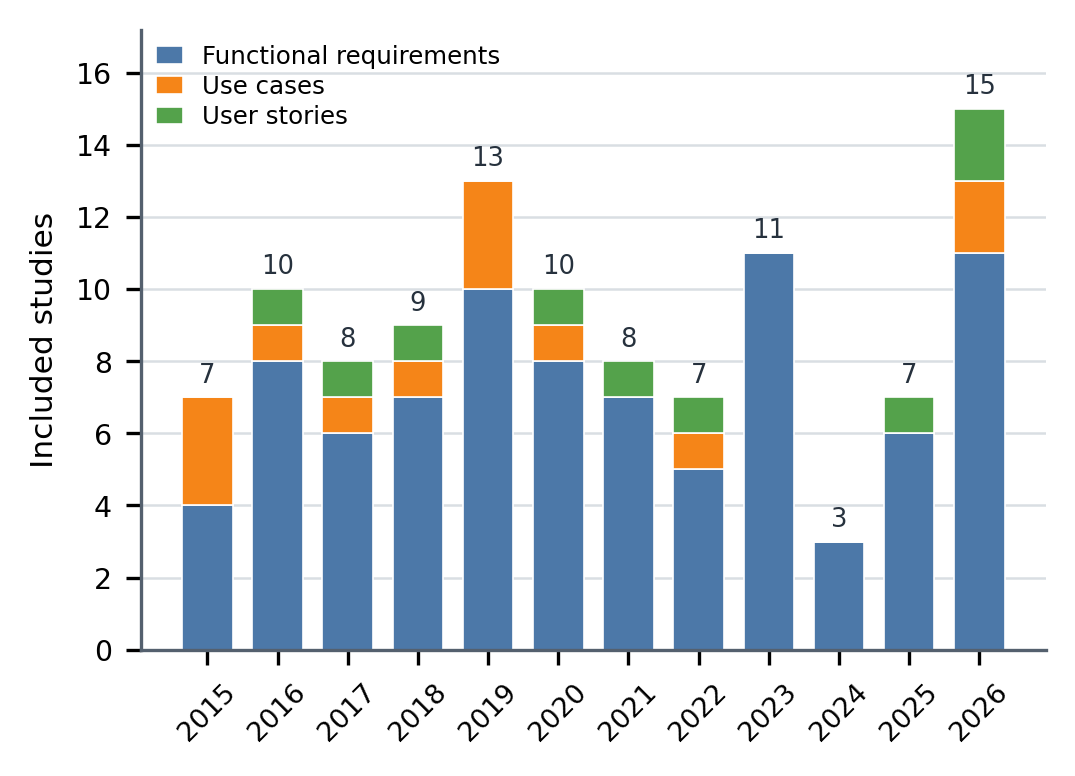
\includegraphics[width=\columnwidth]{fig_years.png}
        \caption{Temporal distribution of the 109 included studies (2015--2026), stacked by requirements-artifact category. The figure above each bar indicates the year's total.}
        \label{fig:years}
    \end{figure}
    
    As Fig.~\ref{fig:years} shows, output on functional requirements holds steady across the whole time window (2015--2026) and accounts for most of the corpus, while the increase observed in the most recent years coincides with the spread of large language models in software engineering. Over this same set of studies, Table~\ref{tab:sintesis} synthesizes the frequencies of standards, notations, and test-derivation techniques observed in the full text, whose analysis is organized below around the four research questions.
    
    \begin{table}[!tb]
        \caption{Synthesis of evidence from the 109 included studies: frequency of standards/notations and of test-derivation techniques (presence in the full text)}
        \label{tab:sintesis}
        \centering
        \small
        \setlength{\tabcolsep}{6pt}
        \begin{tabular}{@{}p{6.9cm}r@{}}
            \toprule
            \textbf{Specification standard / notation} & \textbf{\%} \\
            \midrule
            UML models (use case, sequence, state machine diagrams) & 66 \\
            User story narrative (role--goal, 3C) & 36 \\
            Gherkin / BDD (\emph{Given--When--Then}) & 33 \\
            TDD / ATDD (executable acceptance criteria) & 25 \\
            Controlled natural language (CNL) & 22 \\
            Use case templates (Cockburn / RUCM) & 20 \\
            Acceptance criteria & 20 \\
            Requirements ontologies & 17 \\
            EARS (functional requirements) & 10 \\
            INVEST (user stories) & 6 \\
            ISO/IEC/IEEE 29148 (normative framework) & 5 \\
            \midrule
            \textbf{Test-derivation technique} & \textbf{\%} \\
            \midrule
            Formalization / templates / grammars & 77 \\
            Natural language processing (NLP) & 44 \\
            Model-based testing (MBT) & 41 \\
            Large language models (LLM) & 24 \\
            Ontologies / semantic web & 17 \\
            \bottomrule
        \end{tabular}
        \\[3pt]
        {\footnotesize Frequencies were computed over the 109 included studies and reflect the presence of each standard, notation, or technique detected in the full-text analysis. Abbreviations: UML, \emph{Unified Modeling Language}; BDD, \emph{behavior-driven development}; ATDD, \emph{acceptance test-driven development}; RUCM, \emph{Restricted Use Case Modeling}; EARS, \emph{Easy Approach to Requirements Syntax}. The categories are not mutually exclusive.}
    \end{table}
    
    \textit{RQ1 (standards for structured capture).} The evidence shows that no single normative standard governs practice; instead, each type of specification is structured through a predominant notation. Use cases are captured mostly with UML models---use case, sequence, or state machine diagrams, present in 66\% of the studies \cite{Kudo2019Conceptual,Sandhu2026Framework,Bunder2019Model,Agrawal2023Requirements,Gupta2019Software,Mahanto2018Achieving,Kudo2023Aligning,Intana2023Approach,Intana2023Automated,Orekhov2026Example,Roldan2019Ontology,Abdeen2023Approach,Oran2017Analysing,Fredericks2015Automated,Fischbach2019Automated,Olajubu2018Automated,Bhatia2025Automated,Jang2021Automatic,Nogueira2016Automatic,Jang2025Automatic,Liu2022Automatic,Wiecher2021Besos,Ansari2017Constructing,Arruda2026Deriving,Liu2022Ears2tf,Silva2021Empirical,Tatale2020Enhancing,RochaSilva2020Ensuring,DosSantos2019Extraction,Trinh2026Fstg,Paiva2020Requirements,Zheng2021Generating,Ishinari2025Improving,Chernorutsky2018Industrial,Jorge2018Integrating,Louzaoui2016Invalid,Veizaga2020Leveraging,Zafar2021Model,Carvalho2016Modelling,Miranda2020Preliminary,Yue2015Rtcm,Crapo2017Requirements,Sinha2015Requirements,Wei2024Requirements,Baxter2023Roboworld,Osama2021Srcm,Wiecher2020Scenarios,Khamaiseh2017Software,Bandyszak2015Supporting,Wiecher2019Test,RochaSilva2022Towards,Zafar2021Towards,Clerissi2017Towards,Varpe2025User,Pudlitz2020What,Li2026Test,Tiwari2015Approach,Wang2022Automatic,Wang2015Automatic,Palshikar2019Extraction,Hamza2020Generating,Erazo2017Maritaca,Mai2019Mcp,Diniz2019Reducing,Zhang2018Specifying,Trinh2026Tcg,Wang2015Umtg,Malik2020Automating,Ecar2018Cosmic,Gralha2021Impact,HolodnikJanczura2017Extension,Lucassen2016Use}---and with Cockburn-style templates or their RUCM formalization (20\%)~\cite{Rodriguez2023Behaviour,Roldan2019Ontology,CorreaSouza2018Automated,Oran2017Analysing,Trinh2026Fstg,Paiva2020Requirements,Araujo2017Generating,Veizaga2020Leveraging,Yue2015Rtcm,Medeiros2019Requirements,Khamaiseh2017Software,Clerissi2017Towards,Li2026Test,Tiwari2015Approach,Wang2022Automatic,Wang2015Automatic,Erazo2017Maritaca,Mai2019Mcp,Zhang2018Specifying,Trinh2026Tcg,Wang2015Umtg,Gralha2021Impact}; functional requirements, with controlled natural language (22\%)~\cite{Kudo2023Aligning,Intana2023Approach,CorreaSouza2018Automated,Fischbach2019Automated,Olajubu2018Automated,Bhatia2025Automated,Nogueira2016Automatic,Arruda2026Deriving,Liu2022Ears2tf,Silva2021Empirical,Charoenreh2020Enhancing,Araujo2017Generating,Veizaga2020Leveraging,Carvalho2016Modelling,Miranda2020Preliminary,Yue2015Rtcm,Franca2026Req2test,Baxter2023Roboworld,Osama2021Srcm,RochaSilva2022Towards,Wang2022Automatic,Zhang2018Specifying,Malik2020Automating,Lim2024Test} and the EARS approach (10\%)~\cite{Sandhu2026Framework,Fischbach2019Automated,Olajubu2018Automated,Liu2022Ears2tf,Veizaga2020Leveraging,Crapo2017Requirements,Wei2024Requirements,Osama2021Srcm,Salari2026Test,Pudlitz2020What,Lim2024Test}; and user stories, with the structured role--goal narrative and the 3C scheme (36\%)~\cite{Rodriguez2023Behaviour,Kudo2019Conceptual,Bunder2019Model,Gupta2019Software,Saraiva2023Adoption,Kudo2023Aligning,Nguyen2023Analysis,Intana2023Approach,Orekhov2026Example,Oran2017Analysing,DosSantos2018Automated,Fischbach2019Automated,Bhatia2025Automated,Martins2024Cm,Frattini2023Cira,Silva2021Empirical,RochaSilva2020Ensuring,Matula2018Enterprise,Paiva2020Requirements,Jorge2018Integrating,Miranda2020Preliminary,Saraiva2023Privacy,Yue2015Rtcm,Franca2026Req2test,Medeiros2019Requirements,Khamaiseh2017Software,Moketar2016Testmereq,RochaSilva2022Towards,Pudlitz2020What,Li2026Test,Wu2022Node,Malik2020Automating,Ecar2018Cosmic,Herwanto2025Enhancing,Baker2026Industrial,Gralha2021Impact,Dilorenzo2026Recommending,HolodnikJanczura2017Extension,Lucassen2016Use}, the INVEST model (6\%)~\cite{Khaldi2026Agentic,Abdeen2023Approach,Jorge2018Integrating,Zafar2021Model,Herwanto2025Enhancing,Lucassen2016Use}, and Gherkin/BDD scenarios (33\%)~\cite{Rodriguez2023Behaviour,Kudo2019Conceptual,Sandhu2026Framework,Bunder2019Model,Saraiva2023Adoption,Kudo2023Aligning,Nguyen2023Analysis,Oran2017Analysing,DosSantos2018Automated,Fischbach2019Automated,Wiecher2021Besos,Martins2024Cm,Arruda2026Deriving,Silva2021Empirical,Tatale2020Enhancing,RochaSilva2020Ensuring,Matula2018Enterprise,Fazzolino2019Feature,Paiva2020Requirements,Jorge2018Integrating,Veizaga2020Leveraging,Zafar2021Model,Campanile2022Evaluation,Saraiva2023Privacy,Yue2015Rtcm,Franca2026Req2test,Baxter2023Roboworld,Wiecher2020Scenarios,Wiecher2019Test,RochaSilva2022Towards,Zafar2021Towards,Clerissi2017Towards,Li2026Test,Wang2022Automatic,Wang2015Automatic,Malik2020Automating}. The ISO/IEC/IEEE~29148:2018 framework acts as an overarching reference, though it is explicitly cited in only a minority of studies (5\%)~\cite{iso29148,Kudo2019Conceptual,Orekhov2026Example,Medeiros2019Requirements,Li2026Test,Baker2026Industrial}. This distribution justifies TDDMachine's support for the three artifacts with their respective predominant structures.
    
    \textit{RQ2 (form features).} From the analysis of the templates described by the included studies, we identified the recurring fields that every form must capture: for functional requirements, name, description, type, acceptance criteria, and priority; for use cases, name, actors, goal, the basic flow, and the alternative flows~\cite{Intana2023Approach,Intana2023Automated,CorreaSouza2018Automated,Nogueira2016Automatic,Trinh2026Fstg,Veizaga2020Leveraging,Saraiva2023Privacy,Yue2015Rtcm,Franca2026Req2test,Khamaiseh2017Software,Clerissi2017Towards,Li2026Test,Tiwari2015Approach,Wang2022Automatic,Wang2015Automatic,Palshikar2019Extraction,Erazo2017Maritaca,Mai2019Mcp,Zhang2018Specifying,Trinh2026Tcg,Wang2015Umtg} together with preconditions and postconditions~\cite{Rodriguez2023Behaviour,Longo2016Web,Kudo2023Aligning,Nguyen2023Analysis,Orekhov2026Example,Roldan2019Ontology,DosSantos2018Automated,Olajubu2018Automated,Jang2025Automatic,Liu2022Automatic,Motwani2019Automatically,Tatale2020Enhancing,RochaSilva2020Ensuring,Trinh2026Fstg,Zheng2021Generating,Chernorutsky2018Industrial,Jorge2018Integrating,Louzaoui2016Invalid,Veizaga2020Leveraging,Fisher2016Making,Zafar2021Model,Saraiva2023Privacy,Yue2015Rtcm,Medeiros2019Requirements,Wen2026Research,Osama2021Srcm,Wiecher2020Scenarios,Khamaiseh2017Software,Moketar2016Testmereq,Zafar2021Towards,Clerissi2017Towards,Liu2016Validating,Pudlitz2020What,Li2026Test,Tiwari2015Approach,Wang2022Automatic,Wang2015Automatic,Erazo2017Maritaca,Mai2019Mcp,Diniz2019Reducing,Zhang2018Specifying,Trinh2026Tcg,Wang2015Umtg,Malik2020Automating}; and for user stories, the structured narrative ``as a~[role], I want~[goal], so that~[benefit]''~\cite{Rodriguez2023Behaviour,Kudo2019Conceptual,Bunder2019Model,Gupta2019Software,Saraiva2023Adoption,Kudo2023Aligning,Nguyen2023Analysis,Intana2023Approach,Orekhov2026Example,Oran2017Analysing,DosSantos2018Automated,Fischbach2019Automated,Bhatia2025Automated,Martins2024Cm,Frattini2023Cira,Silva2021Empirical,RochaSilva2020Ensuring,Matula2018Enterprise,Paiva2020Requirements,Jorge2018Integrating,Miranda2020Preliminary,Saraiva2023Privacy,Yue2015Rtcm,Franca2026Req2test,Medeiros2019Requirements,Khamaiseh2017Software,Moketar2016Testmereq,RochaSilva2022Towards,Pudlitz2020What,Li2026Test,Wu2022Node,Malik2020Automating,Ecar2018Cosmic,Herwanto2025Enhancing,Baker2026Industrial,Gralha2021Impact,Dilorenzo2026Recommending,HolodnikJanczura2017Extension,Lucassen2016Use} along with their acceptance criteria~\cite{Rodriguez2023Behaviour,Gupta2019Software,Nguyen2023Analysis,Orekhov2026Example,DosSantos2018Automated,Fischbach2019Automated,Olajubu2018Automated,Frattini2023Cira,Silva2021Empirical,Tatale2020Enhancing,RochaSilva2020Ensuring,Paiva2020Requirements,Veizaga2020Leveraging,Franca2026Req2test,Medeiros2019Requirements,Khamaiseh2017Software,RochaSilva2022Towards,Li2026Test,Malik2020Automating,Baker2026Industrial,Dilorenzo2026Recommending,HolodnikJanczura2017Extension}. These fields, matching the canonical Cockburn templates and their RUCM formalization~\cite{Rodriguez2023Behaviour,Roldan2019Ontology,CorreaSouza2018Automated,Oran2017Analysing,Trinh2026Fstg,Paiva2020Requirements,Araujo2017Generating,Veizaga2020Leveraging,Yue2015Rtcm,Medeiros2019Requirements,Khamaiseh2017Software,Clerissi2017Towards,Li2026Test,Tiwari2015Approach,Wang2022Automatic,Wang2015Automatic,Erazo2017Maritaca,Mai2019Mcp,Zhang2018Specifying,Trinh2026Tcg,Wang2015Umtg,Gralha2021Impact}, the ISO/IEC/IEEE~29148 standard, and the INVEST/Connextra model, were implemented as mandatory in the tool; those appearing in a minority of sources (status, source, dependencies, or estimation) were made optional.
    
    \textit{RQ3 (relationship with test generation).} Techniques that exploit structured or formalized input predominate: formalization through templates, grammars, or controlled natural language appears in 77\% of the studies \cite{Rodriguez2023Behaviour,Morales2024Dsl,Sandhu2026Framework,Bunder2019Model,Agrawal2023Requirements,Khaldi2026Agentic,Kudo2023Aligning,Intana2023Approach,Orekhov2026Example,Roldan2019Ontology,Abdeen2023Approach,CorreaSouza2018Automated,Oran2017Analysing,Fredericks2015Automated,Fischbach2019Automated,Olajubu2018Automated,Bhatia2025Automated,Jang2021Automatic,Nogueira2016Automatic,Jang2025Automatic,Liu2022Automatic,Motwani2019Automatically,Wiecher2021Besos,Martins2024Cm,Ansari2017Constructing,Venkatesh2016Cost,Arruda2026Deriving,Liu2022Ears2tf,Silva2021Empirical,Charoenreh2020Enhancing,RochaSilva2020Ensuring,Matula2018Enterprise,DosSantos2019Extraction,Trinh2026Fstg,Paiva2020Requirements,Araujo2017Generating,Zheng2021Generating,Chernorutsky2018Industrial,Jorge2018Integrating,Veizaga2020Leveraging,Zafar2021Model,Carvalho2016Modelling,Campanile2022Evaluation,Miranda2020Preliminary,Saraiva2023Privacy,Borg2022Quality,LeonQuinstedt2026Rest,Yue2015Rtcm,Franca2026Req2test,Crapo2017Requirements,Sinha2015Requirements,Medeiros2019Requirements,Wen2026Research,Baxter2023Roboworld,Osama2021Srcm,Wiecher2020Scenarios,Khamaiseh2017Software,Bandyszak2015Supporting,Wiecher2019Test,Moketar2016Testmereq,RochaSilva2022Towards,Zafar2021Towards,Clerissi2017Towards,Varpe2025User,Pudlitz2020What,Li2026Test,Tiwari2015Approach,Wang2022Automatic,Wang2015Automatic,Palshikar2019Extraction,Erazo2017Maritaca,Mai2019Mcp,Zhang2018Specifying,Trinh2026Tcg,Wang2015Umtg,Wu2022Node,Malik2020Automating,Ecar2018Cosmic,Herwanto2025Enhancing,Gralha2021Impact,Dilorenzo2026Recommending,HolodnikJanczura2017Extension,Lucassen2016Use,Lim2024Test}; natural language processing, in 44\%~\cite{Morales2024Dsl,Sandhu2026Framework,Bunder2019Model,Intana2023Approach,Fathima2026Automated,Olajubu2018Automated,Bhatia2025Automated,Jang2025Automatic,Motwani2019Automatically,Frattini2023Cira,Ansari2017Constructing,Ishinari2026Data,Arruda2026Deriving,Liu2022Ears2tf,Silva2021Empirical,Charoenreh2020Enhancing,RochaSilva2020Ensuring,Trinh2026Fstg,Araujo2017Generating,Zheng2021Generating,Ishinari2025Improving,Veizaga2020Leveraging,Campanile2022Evaluation,Miranda2020Preliminary,Borg2022Quality,LeonQuinstedt2026Rest,Franca2026Req2test,Wei2024Requirements,Wen2026Research,Baxter2023Roboworld,Osama2021Srcm,RochaSilva2022Towards,Clerissi2017Towards,Pudlitz2020What,Li2026Test,Wang2022Automatic,Wang2015Automatic,Palshikar2019Extraction,Erazo2017Maritaca,Mai2019Mcp,Zhang2018Specifying,Trinh2026Tcg,Wang2015Umtg,Wu2022Node,Malik2020Automating,Herwanto2025Enhancing,Gralha2021Impact,Lim2024Test}; model-based testing, in 41\%~\cite{Morales2024Dsl,Sandhu2026Framework,Bunder2019Model,Roldan2019Ontology,Abdeen2023Approach,DosSantos2018Automated,Fredericks2015Automated,Fischbach2019Automated,Olajubu2018Automated,Bhatia2025Automated,Jang2021Automatic,Nogueira2016Automatic,Jang2025Automatic,Liu2022Automatic,Venkatesh2016Cost,Liu2022Ears2tf,Tatale2020Enhancing,RochaSilva2020Ensuring,DosSantos2019Extraction,Trinh2026Fstg,Fazzolino2019Feature,Paiva2020Requirements,Zheng2021Generating,Jorge2018Integrating,Zafar2021Model,Carvalho2016Modelling,Miranda2020Preliminary,Yue2015Rtcm,Franca2026Req2test,Baxter2023Roboworld,Khamaiseh2017Software,Bandyszak2015Supporting,Zafar2021Towards,Clerissi2017Towards,Varpe2025User,Pudlitz2020What,Tiwari2015Approach,Wang2022Automatic,Wang2015Automatic,Hamza2020Generating,Erazo2017Maritaca,Diniz2019Reducing,Zhang2018Specifying,Wang2015Umtg,Malik2020Automating}; and the use of large language models, in 24\%~\cite{Morales2024Dsl,Khaldi2026Agentic,Orekhov2026Example,Fathima2026Automated,Bhatia2025Automated,Jang2025Automatic,Shimizu2025Automatic,Ishinari2026Data,Arruda2026Deriving,Trinh2026Fstg,Ishinari2025Improving,Louzaoui2016Invalid,Borg2022Quality,LeonQuinstedt2026Rest,Franca2026Req2test,Sinha2015Requirements,Wei2024Requirements,Wen2026Research,Salari2026Test,Varpe2025User,Li2026Test,Trinh2026Tcg,Wu2022Node,Herwanto2025Enhancing,Baker2026Industrial,Dilorenzo2026Recommending}, with a rising trend in the most recent years. Structured fields---particularly acceptance criteria and pre/postconditions---translate directly into verifiable assertions, so standardizing the input reduces the ambiguity of natural language and improves the consistency of the automatically generated tests, in line with evidence that the quality of the input specification determines that of the output \cite{wang2024survey,yang2024evaluation}.
    
    \textit{RQ4 (existing CASE tools).} The tools identified fall into two families. The first derives tests from structured requirements specifications---for example, generators from restricted use cases (RUCM/UMTG, aToucan, MARITACA), from natural-language requirements (CiRA, TestMEReq, EARS2TF), and, in the most recent work, LLM-assisted ones (Req2Test, REST-at)~\cite{Morales2024Dsl,Khaldi2026Agentic,Orekhov2026Example,Fathima2026Automated,Bhatia2025Automated,Jang2025Automatic,Shimizu2025Automatic,Ishinari2026Data,Arruda2026Deriving,Trinh2026Fstg,Ishinari2025Improving,Louzaoui2016Invalid,Borg2022Quality,LeonQuinstedt2026Rest,Franca2026Req2test,Sinha2015Requirements,Wei2024Requirements,Wen2026Research,Salari2026Test,Varpe2025User,Li2026Test,Trinh2026Tcg,Wu2022Node,Herwanto2025Enhancing,Baker2026Industrial,Dilorenzo2026Recommending}---but it usually stops at the test specification without covering the TDD cycle. The second generates tests from source code or free text---\emph{ChatUniTest} \cite{chen2024chatunitest}, \emph{TestSpark} \cite{sapozhnikov2024testspark}, \emph{Pynguin} \cite{lukasczyk2022pynguin}, and \emph{Pytester} \cite{takerngsaksiri2025pytester}---so it operates at a later phase, in a \emph{test-last} scheme. None integrates the structured capture of requirements with the LLM-assisted generation of the \emph{Red}-stage test, a gap that TDDMachine addresses. The analysis further shows that general-purpose models with strong capabilities for synthesis and code processing---Claude 3.5 Sonnet and GPT-4---were the ones preferred in recent literature, in line with Hou et~al.'s review of LLMs for software engineering \cite{hou2024llm4se}.
    
    \subsection{Positioning Against the State of the Art}
    \label{subsec:posicionamiento}
    
    To position the contribution against a broad set of systems, Table~\ref{tab:comparacion} contrasts TDDMachine with fourteen representative state-of-the-art tools, grouped into three families: (i)~test generators from structured requirements specifications---restricted use cases with UMTG \cite{Wang2015Umtg}, RTCM/aToucan \cite{Yue2015Rtcm}, MARITACA \cite{Erazo2017Maritaca}, and acceptance-test generation from use cases \cite{Wang2022Automatic}; natural-language requirements with CiRA \cite{Frattini2023Cira}, TestMEReq \cite{Moketar2016Testmereq}, EARS2TF \cite{Liu2022Ears2tf}, and requirements-to-test-case conversion \cite{Gupta2019Software}---; (ii)~recent LLM-assisted proposals---Req2Test \cite{Franca2026Req2test} and REST-at \cite{LeonQuinstedt2026Rest}---; and (iii)~generators that start from source code or free text---\emph{ChatUniTest} \cite{chen2024chatunitest}, \emph{TestSpark} \cite{sapozhnikov2024testspark}, \emph{Pynguin} \cite{lukasczyk2022pynguin}, and \emph{Pytester} \cite{takerngsaksiri2025pytester}. The comparison shows that requirements-based tools rarely integrate an LLM engine and none incorporates AST validation of the generated code or the management and export of the test cycle; LLM-based tools do not capture the three artifact types in a structured way; and code-oriented tools operate in a \emph{test-last} scheme, once production code already exists. TDDMachine is the only proposal that brings together structured capture of the three artifacts, an LLM engine, AST syntactic validation, and integrated management, while placing itself explicitly at the \emph{Red} stage of the TDD cycle.
    
    \begin{table*}[!tb]
        \caption{Comparison of TDDMachine with fourteen representative state-of-the-art tools}
        \label{tab:comparacion}
        \centering
        \small
        \setlength{\tabcolsep}{5pt}
        \begin{tabular}{@{}lccccc@{}}
            \toprule
            \textbf{Tool} & \textbf{Input\textsuperscript{a}} & \textbf{Artifact} & \textbf{Engine\textsuperscript{b}} & \textbf{AST valid.} & \textbf{Mgmt.\textsuperscript{c}} \\
            \midrule
            \textbf{TDDMachine (this work)} & SR & FR, UC, US & LLM & Yes & Yes \\
            \midrule
            \multicolumn{6}{@{}l}{\textit{Generators from structured requirements specifications}} \\
            UMTG \cite{Wang2015Umtg}            & SR & UC        & NLP     & No & Partial \\
            RTCM / aToucan \cite{Yue2015Rtcm}   & SR & UC        & NLP     & No & No \\
            Acceptance tests from UC \cite{Wang2022Automatic} & SR & UC & NLP & No & No \\
            MARITACA \cite{Erazo2017Maritaca}   & SR & UC        & NLP/MBT & No & No \\
            CiRA \cite{Frattini2023Cira}        & NL & FR        & NLP/ML  & No & Partial \\
            TestMEReq \cite{Moketar2016Testmereq} & SR & FR      & MBT     & No & No \\
            EARS2TF \cite{Liu2022Ears2tf}       & SR & FR        & Semiformal & No & No \\
            Convert requirements to tests \cite{Gupta2019Software} & SR & FR & NLP & No & No \\
            \midrule
            \multicolumn{6}{@{}l}{\textit{LLM-assisted proposals}} \\
            Req2Test \cite{Franca2026Req2test}  & SR & US        & LLM     & No & Partial \\
            REST-at \cite{LeonQuinstedt2026Rest} & SR & FR       & LLM     & No & Partial \\
            \midrule
            \multicolumn{6}{@{}l}{\textit{Generators from source code or free text (\emph{test-last})}} \\
            ChatUniTest \cite{chen2024chatunitest}      & SC & ---   & LLM    & Partial & Partial \\
            TestSpark \cite{sapozhnikov2024testspark}   & SC & ---   & LLM/EV & Partial & Yes \\
            Pynguin \cite{lukasczyk2022pynguin}         & SC & ---   & EV     & Yes   & No \\
            Pytester \cite{takerngsaksiri2025pytester}  & FT & ---   & RL     & No    & No \\
            \bottomrule
        \end{tabular}
        \\[3pt]
        {\footnotesize \textsuperscript{a}\,Input: SR\,=\,structured requirements; NL\,=\,natural-language requirements; SC\,=\,source code; FT\,=\,free text. \textsuperscript{b}\,Engine: LLM\,=\,large language model; NLP\,=\,natural language processing; MBT\,=\,model-based testing; EV\,=\,evolutionary algorithms; RL\,=\,reinforcement learning; ML\,=\,machine learning. \textsuperscript{c}\,Mgmt.\,=\,integrated review, editing, and export capabilities for the test cycle. Only TDDMachine intervenes explicitly at the \emph{Red} stage of the TDD cycle (before production code exists). FR\,=\,functional requirements; UC\,=\,use cases; US\,=\,user stories.}
    \end{table*}
    
    \subsection{Threats to the Validity of the Review}
    \label{subsec:amenazas}
    
    The review has the usual limitations of a bounded SLR. Construct validity is conditioned by the restriction to four databases (Scopus, IEEE~Xplore, ACM~Digital~Library, and Web of Science) and to English-language publications from 2015 onward, which may have left out relevant literature in other sources or languages; this was mitigated with search strings built on the PICOC approach---with truncation and synonyms to maximize coverage---and complemented by a search of open-source repositories. To bound the risk of selection bias, screening and extraction followed a multi-author review protocol: the second author performed the initial selection of studies; the first author reviewed the process step by step to confirm and correct the decisions; and the third, fourth, and fifth authors carried out a full review of the process. Disagreements were resolved by consensus and, failing that, by majority among the five authors. This procedure, together with the application of explicit inclusion and exclusion criteria, a standardized extraction template, and a documented record of the reasons for exclusion, mitigates single-reviewer bias and strengthens the reliability of the selection. Internal validity nonetheless retains the limitation inherent to the human interpretation of the criteria, attenuated by triangulation among reviewers.
    
    %% ------------------------------------------------------------------------
    \section{Methodology}
    \label{sec:metodologia}
    
    TDDMachine was developed in six successive phases---requirements analysis, specification, architectural design, module implementation, verification and validation, and deployment---under a Component-Based Software Engineering (CBSE) approach. The tool's scope was delimited explicitly: it intervenes only in the \emph{Red}$\rightarrow$\emph{Green} transition of the TDD cycle, generating the test script that the development team will use as the initial state; the \emph{Green} and \emph{Refactor} stages fall outside its scope. Accordingly, the supported language is Python and the testing framework is \texttt{pytest}.
    
    \subsection{Design and Development of the Tool}
    \label{subsec:desarrollo}
    
    The requirements were derived from the systematic review described in Section~\ref{sec:trabajos}: from the fields identified in the templates of the included studies and in the reference standards, we determined what information to capture in each form, classifying as mandatory the recurring fields---those consistently present in those templates---and as optional the rest. This analysis yielded eighteen functional requirements organized into four modules---authentication and user management, project management, specification capture, and test generation and management---and a set of non-functional requirements for security, performance, usability, integration, and availability, specified in accordance with ISO/IEC/IEEE~29148:2018 and ISO/IEC~25010 \cite{iso29148}. The technology components were selected through a weighted multi-criteria decision matrix, in which each alternative was rated from 1 to 5 on technical criteria with percentage weights; the selection resulted in React~18 with Ant~Design on the frontend, Django~4.2 with Django REST Framework on the backend, PostgreSQL~15 as the database manager, and Claude 3.5 Sonnet as the generation model.
    
    On these requirements we built a client--server architecture organized into four layers with well-defined interfaces---presentation, business logic, persistence, and infrastructure---summarized in Fig.~\ref{fig:arquitectura}. The React~18 frontend communicates with the Django backend through a REST-style (Representational State Transfer) application programming interface (API), whose interceptors attach the JWT (JSON Web Token) authentication token to every request. The business-logic layer implements three main services that realize the generation flow: \texttt{PromptBuilder}, which builds structured prompts from the type and content of each specification; \texttt{ClaudeService}, which manages the calls to the Anthropic API with automatic retries and exponential backoff on transient failures; and \texttt{PytestValidator}, which checks the syntax of the generated code by analyzing Python's abstract syntax tree (AST). This separation isolates prompt construction, model invocation, and syntactic quality control, so that each stage can evolve or be replaced independently. To support reproducibility, \texttt{ClaudeService} invoked the model with version \texttt{\llmversion}, temperature \texttt{\llmtemperatura}, and an output-token limit of \texttt{\llmmaxtokens}, over a 200,000-token context window, during the access period \llmperiodo.
    
    \begin{figure}[!tb]
        \centering
        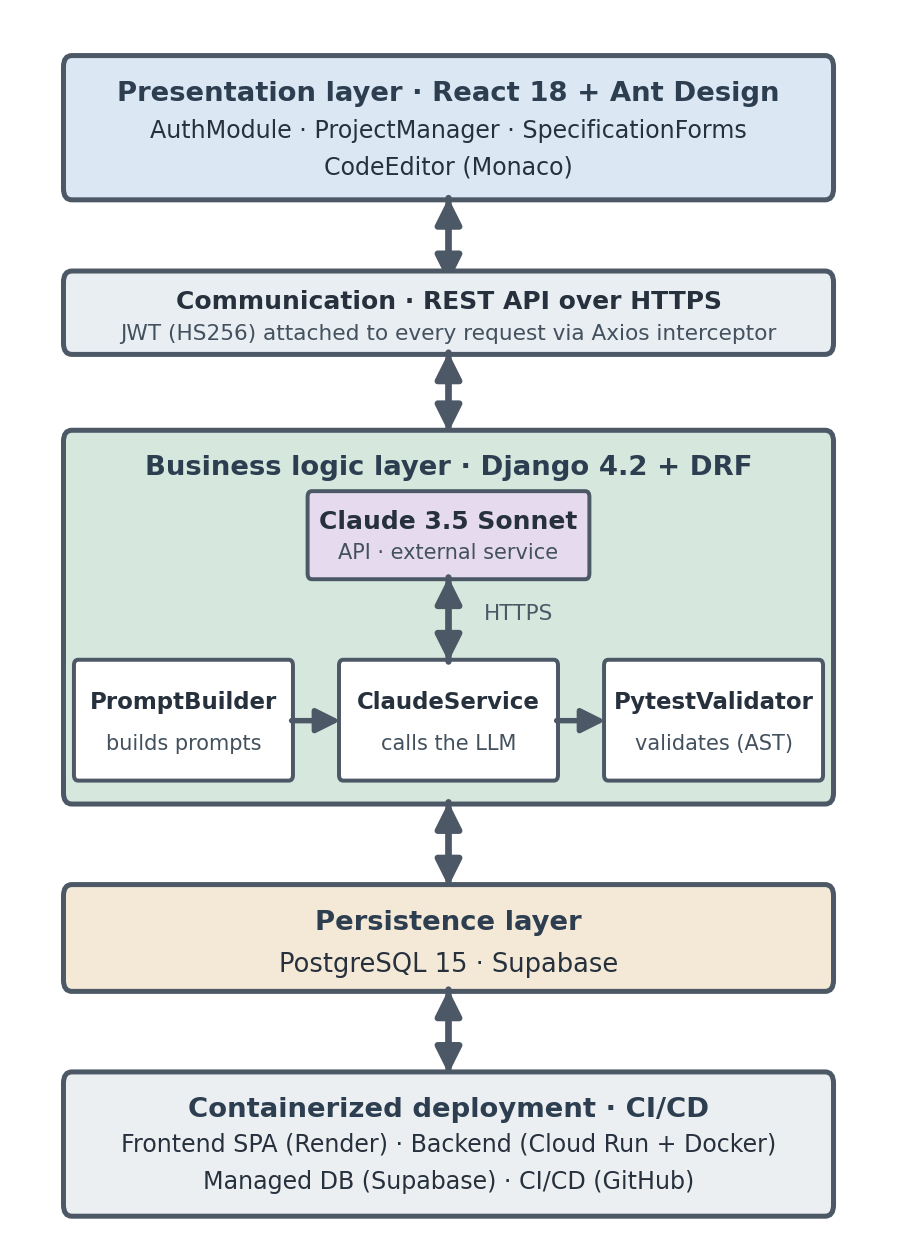
\includegraphics[width=\columnwidth]{fig_arquitectura.png}
        \caption{Layered architecture of TDDMachine. The presentation layer (React~18 with Ant~Design) captures the three specifications and reviews the script in a Monaco editor; the business-logic layer (Django~4.2 with Django REST Framework) chains the \texttt{PromptBuilder}, \texttt{ClaudeService}---the sole integration point with the Claude 3.5 Sonnet API---and \texttt{PytestValidator} services; the persistence layer (PostgreSQL~15 on Supabase) stores projects, specifications, and tests; and the infrastructure layer deploys the backend in a Docker container on Cloud~Run and the frontend as a single-page application on Render.}
        \label{fig:arquitectura}
    \end{figure}
    
    The layered organization in Fig.~\ref{fig:arquitectura}, consistent with the component-based software engineering approach adopted, makes it possible to replace or upgrade each component---for example, the language model in the business-logic layer or the database manager in the persistence layer---without altering the rest of the system.
    
    As for the structure of the generated script, the \texttt{PromptBuilder} service instructs the model to produce \texttt{pytest} tests organized with \emph{fixtures}---pytest's mechanism for setting up and tearing down the test environment (\emph{setup}/\emph{teardown})---and assertions derived from the acceptance criteria of the specification. One aspect specific to the \emph{Red} stage is the handling of external dependencies of code that does not yet exist, in particular database access, LLM invocation, or network communication: the initial test state must isolate the unit under test from those dependencies through \emph{test doubles}. In the Python ecosystem, this isolation is achieved with the standard library \texttt{unittest.mock}---which allows mock objects to be created and dependencies to be substituted through \texttt{patch}, analogous to \emph{Mockito} in Java---and its \texttt{pytest} wrapper, the \texttt{pytest-mock} plugin (\emph{fixture} \texttt{mocker}); for tests that must exercise the persistence layer, the \texttt{pytest-django} plugin provides a transactional test database through the \texttt{db} \emph{fixture}. Accordingly, the \texttt{PromptBuilder} guidelines cover the generation of \emph{fixtures} and, when the specification involves data access, the mocking of those dependencies; strengthening the automatic generation of \emph{mocks} and \emph{fixtures} for complex data dependencies is one of the improvement areas identified in the expert evaluation.
    
    The validation outcome determines how each test is handled: when it succeeds, the test is stored with the status ``Generated''; on a syntax error, it is recorded with the status ``Generation error'' and still presented to the user for manual correction in an integrated Monaco editor with syntax highlighting, autocompletion, and real-time error detection. The management module lets users review, classify (Generated, Reviewed, Approved, Discarded), and export the approved tests as a downloadable \texttt{.py} file. Deployment was carried out on cloud infrastructure---frontend on Render, backend in a Docker container on Cloud Run, and a managed PostgreSQL database on Supabase, with continuous integration from the project's GitHub repository.
    
    \subsection{Evaluation Design}
    \label{subsec:validacion}
    
    The evaluation was structured into two complementary studies, designed to match the tool's scope. Study~1, on usability and technology acceptance, involved the voluntary participation of 25 sixth-semester Software Engineering students, who completed four tasks covering the \emph{Red}-stage flow: creating a project and registering a use case, specifying a functional requirement, writing a user story, and generating, reviewing, and exporting the \texttt{pytest} script. Usability was measured with the SUS (System Usability Scale), a standardized 10-item questionnaire on a 5-point Likert scale whose score is transformed to a 0--100 scale and interpreted according to the adjective scale of Bangor et~al. \cite{brooke1996sus,bangor2009sus}. Technology acceptance was measured with an instrument based on the TAM (Technology Acceptance Model), comprising 16 items across four constructs---Perceived Usefulness (PU), Perceived Ease of Use (PEOU), Confidence in Results (CR), and Intention to Use (IU)---with an acceptance threshold of 3.5/5 per construct \cite{davis1989tam}.
    
    Study~2, on test quality, involved 10 testing experts who used a structured rubric, on a 1-to-5 scale, to assess five criteria---completeness, clarity, traceability, execution feasibility, and scenario coverage---over 15 generated test cases. Beyond the structural review of each script, execution feasibility was checked by running the generated tests against the production code hosted in the project's public repositories: the experts confirmed that every script failed on its first run---the expected behavior of the \emph{Red} stage, in which no implementation yet exists---and passed once the corresponding minimum code was added (the \emph{Green} stage), which made it possible to verify their functional correctness and not merely their syntactic validity.
    
    %% ------------------------------------------------------------------------
    \section{Results}
    \label{sec:resultados}
    
    \subsection{Effectiveness of Automatic Generation}
    \label{subsec:generacion}
    
    During the evaluation phase, 70 attempts to generate \texttt{pytest} scripts from the captured specifications were recorded. Table~\ref{tab:generacion} summarizes the results by specification type: the overall rate of valid scripts was 91.4\%, with the best performance on functional requirements (96.4\%) and the lowest on user stories (83.3\%). The six failed attempts corresponded to errors detected by \texttt{PytestValidator} during AST analysis---in four cases, incomplete code blocks attributable to specifications with ambiguous acceptance criteria, and in two, structural errors in the test function; in all of them the system preserved traceability by recording the test with the status ``Generation error'' for manual correction.
    
    \begin{table}[!tb]
        \caption{Generation of \texttt{pytest} scripts by specification type}
        \label{tab:generacion}
        \centering
        \small
        \begin{tabular}{@{}lcccc@{}}
            \toprule
            \textbf{Specification} & \textbf{Attempts} & \textbf{Valid} & \textbf{Error} & \textbf{Success} \\
            \midrule
            Functional requirements & 28 & 27 & 1 & 96.4\% \\
            Use cases               & 24 & 22 & 2 & 91.7\% \\
            User stories            & 18 & 15 & 3 & 83.3\% \\
            \midrule
            \textbf{Total}          & \textbf{70} & \textbf{64} & \textbf{6} & \textbf{91.4\%} \\
            \bottomrule
        \end{tabular}
    \end{table}
    
    \subsection{Usability and Technology Acceptance}
    \label{subsec:sustam}
    
    The 25 participants completed the four tasks in a mean time of 42.0 minutes (standard deviation, SD\,=\,8.2). The mean SUS score was 74.46/100 (SD\,=\,6.55; minimum 62.5; maximum 85.0), which exceeds the ``Good'' threshold (68 points) on the Bangor et~al. scale and places the tool above the average of the systems evaluated with this instrument \cite{bangor2009sus}. As for technology acceptance, Table~\ref{tab:tam} presents the descriptive statistics and reliability by TAM construct.
    
    \begin{table}[!tb]
        \caption{Descriptive statistics and reliability by TAM construct (n\,=\,25)}
        \label{tab:tam}
        \centering
        \small
        \setlength{\tabcolsep}{3pt}
        \begin{tabular}{@{}lccccc@{}}
            \toprule
            \textbf{Construct} & \textbf{Items} & \textbf{Mean} & \textbf{SD} & \textbf{$\alpha$} & \textbf{Interp.} \\
            \midrule
            Perceived Usefulness (PU)   & 5 & 4.14 & 0.56 & 0.847 & High \\
            Perceived Ease of Use (PEOU) & 4 & 4.02 & 0.63 & 0.812 & High \\
            Confidence in Results (CR)  & 4 & 3.76 & 0.71 & 0.798 & Mod.--High \\
            Intention to Use (IU)       & 3 & 4.08 & 0.60 & 0.831 & High \\
            \midrule
            \textbf{Overall}            & \textbf{16} & \textbf{4.00} & \textbf{0.63} & \textbf{0.883} & \textbf{High} \\
            \bottomrule
        \end{tabular}
    \end{table}
    
    As Table~\ref{tab:tam} shows, the four constructs exceeded the 3.5/5 threshold: Perceived Usefulness (4.14) and Intention to Use (4.08) obtained the highest values, while Confidence in Results (3.76) was the construct closest to the threshold, reflecting participants' uncertainty about the reliability of AI-generated code. The instrument showed adequate internal consistency, with an overall Cronbach's alpha of 0.883 and per-construct values above 0.79. The participant-level evidence is summarized in Fig.~\ref{fig:sustam}, which brings together the distribution of individual SUS scores (a) and the Pearson correlation matrix among the TAM constructs (b).
    
    \begin{figure}[!tb]
        \centering
        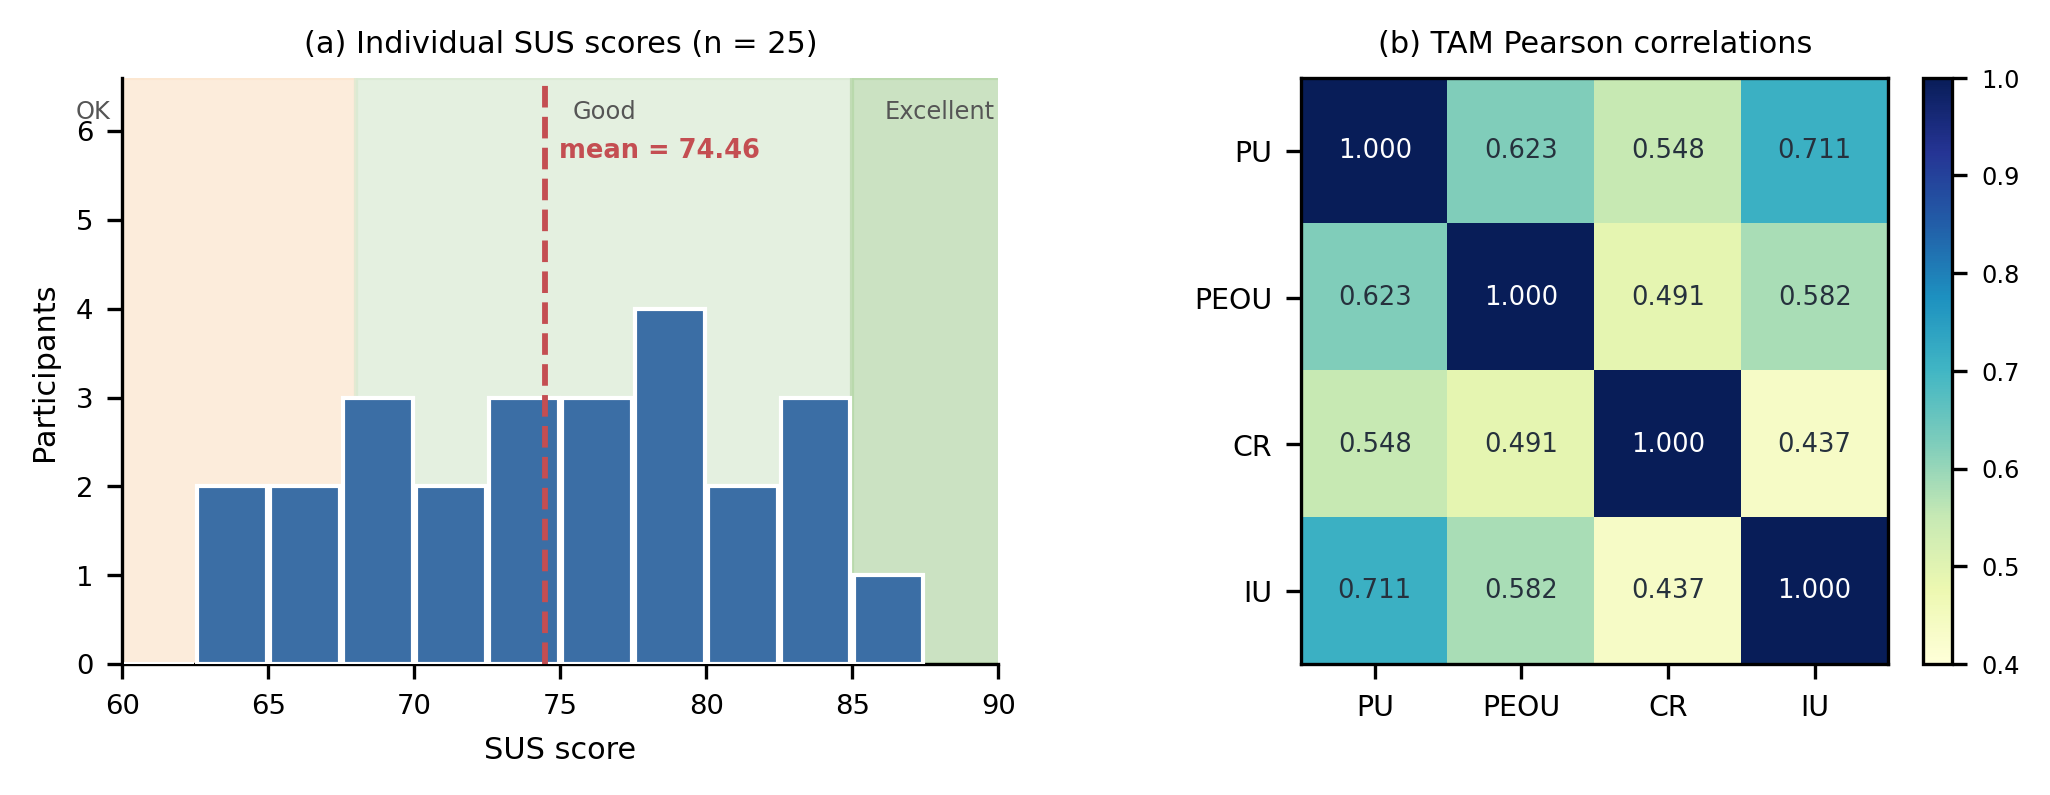
\includegraphics[width=\columnwidth]{fig_sus_tam.png}
        \caption{Results of the usability and technology-acceptance study (n\,=\,25). (a)~Distribution of individual SUS scores over the interpretive bands of the Bangor et~al. scale; the dashed line marks the mean (74.46). (b)~Pearson correlation matrix among the four TAM constructs; color intensity represents the magnitude of the coefficient.}
        \label{fig:sustam}
    \end{figure}
    
    The distribution in Fig.~\ref{fig:sustam}(a) indicates that 80\% of the participants (20 of 25) reached at least the ``Good'' threshold (SUS\,$\geq$\,68), with no case below the minimum acceptable level of the scale. The correlation map in Fig.~\ref{fig:sustam}(b), in turn, shows that all associations among constructs are positive and statistically significant (p\,<\,0.05), and that the strongest occurs between Perceived Usefulness and Intention to Use (r\,=\,0.711; p\,<\,0.01), confirming the central assumption of the TAM.
    
    \subsection{Quality of the Generated Tests}
    \label{subsec:calidad}
    
    The expert evaluation yielded an overall mean quality of 4.08/5.0 across the five rubric criteria. Table~\ref{tab:calidad} presents the mean rating, standard deviation, and interpretation by criterion.
    
    \begin{table}[!tb]
        \caption{Test quality by criterion (1--5 scale, n\,=\,10 experts)}
        \label{tab:calidad}
        \centering
        \small
        \begin{tabular}{@{}lccc@{}}
            \toprule
            \textbf{Criterion} & \textbf{Mean} & \textbf{SD} & \textbf{Interpretation} \\
            \midrule
            Completeness          & 4.2 & 0.45 & Very good \\
            Clarity               & 4.3 & 0.42 & Very good \\
            Traceability          & 4.0 & 0.58 & Good \\
            Execution feasibility & 3.9 & 0.67 & Good \\
            Scenario coverage     & 4.0 & 0.61 & Good \\
            \midrule
            \textbf{Overall mean} & \textbf{4.08} & \textbf{0.55} & \textbf{Very good} \\
            \bottomrule
        \end{tabular}
    \end{table}
    
    According to Table~\ref{tab:calidad}, the best-rated criteria were clarity (4.3) and completeness (4.2), rated ``Very good,'' while execution feasibility (3.9) was the criterion closest to the threshold, which points to room for improvement in the precision of the assertions relative to the conditions of the source specification. Broken down by test type, the unit tests generated from functional requirements reached the highest quality (4.24), followed by integration tests from use cases (4.08) and system tests from user stories (3.92). Figure~\ref{fig:gradient} relates this breakdown to the generation validity of Table~\ref{tab:generacion} by the type of source requirements artifact.
    
    \begin{figure}[!tb]
        \centering
        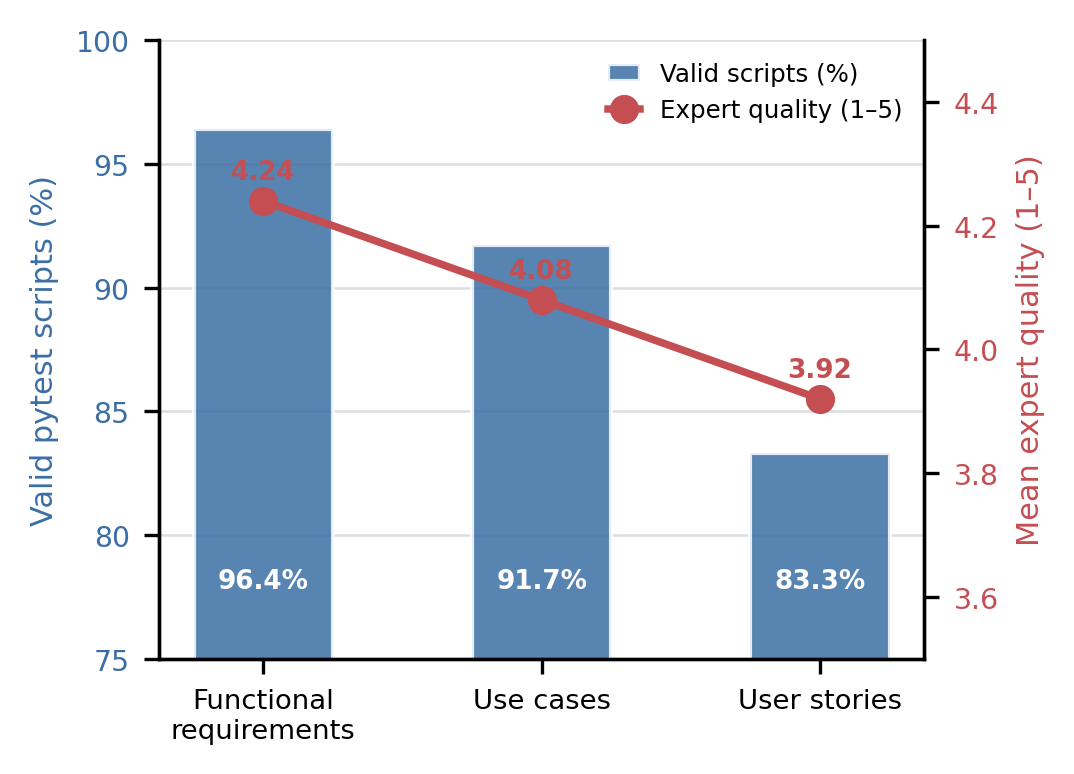
\includegraphics[width=\columnwidth]{fig_gradient.png}
        \caption{Generation validity of \texttt{pytest} scripts (Table~\ref{tab:generacion}) and mean expert quality of the tests (Table~\ref{tab:calidad}) by the type of source requirements artifact. Both indicators decline in step from functional requirements toward user stories, as the ambiguity of the specification increases.}
        \label{fig:gradient}
    \end{figure}
    
    As Fig.~\ref{fig:gradient} shows, both indicators follow a matching trend: moving from functional requirements to use cases and to user stories---that is, as the specification becomes less structured and more ambiguous---the proportion of valid scripts falls from 96.4\% to 91.7\% and to 83.3\%, and expert quality falls from 4.24 to 4.08 and to 3.92. This concordance suggests that the degree of structure of the requirements artifact is a common determinant of both generation success and the quality of the resulting tests.
    
    Beyond the rubric scores, execution feasibility was corroborated functionally by running the generated tests against the project's production code: every script failed on its first run---the correct behavior of the \emph{Red} stage, before any implementation exists---and passed after the minimum \emph{Green}-stage code was added, which shows that the scripts are not only syntactically valid but also functionally correct as an initial test state. In the qualitative questionnaire, the experts informally compared the generated tests with those they would write by hand and agreed that the tool reproduces the tests expected for each specification and, in several cases, proposes relevant additional scenarios they had not anticipated; among the areas for improvement, they pointed to strengthening the negative and boundary-value scenarios, a recommendation taken up in the future-work lines.
    
    %% ------------------------------------------------------------------------
    \section{Discussion}
    \label{sec:discusion}
    
    The findings of this work are interpreted in light of the body of 109 primary studies included in the systematic review \cite{Kudo2019Conceptual,Sandhu2026Framework,Bunder2019Model,Agrawal2023Requirements,Gupta2019Software,Mahanto2018Achieving,Kudo2023Aligning,Intana2023Approach,Intana2023Automated,Orekhov2026Example,Roldan2019Ontology,Abdeen2023Approach,Oran2017Analysing,Fredericks2015Automated,Fischbach2019Automated,Olajubu2018Automated,Bhatia2025Automated,Jang2021Automatic,Nogueira2016Automatic,Jang2025Automatic,Liu2022Automatic,Wiecher2021Besos,Ansari2017Constructing,Arruda2026Deriving,Liu2022Ears2tf,Silva2021Empirical,Tatale2020Enhancing,RochaSilva2020Ensuring,DosSantos2019Extraction,Trinh2026Fstg,Paiva2020Requirements,Zheng2021Generating,Ishinari2025Improving,Chernorutsky2018Industrial,Jorge2018Integrating,Louzaoui2016Invalid,Veizaga2020Leveraging,Zafar2021Model,Carvalho2016Modelling,Miranda2020Preliminary,Yue2015Rtcm,Crapo2017Requirements,Sinha2015Requirements,Wei2024Requirements,Baxter2023Roboworld,Osama2021Srcm,Wiecher2020Scenarios,Khamaiseh2017Software,Bandyszak2015Supporting,Wiecher2019Test,RochaSilva2022Towards,Zafar2021Towards,Clerissi2017Towards,Varpe2025User,Pudlitz2020What,Li2026Test,Tiwari2015Approach,Wang2022Automatic,Wang2015Automatic,Palshikar2019Extraction,Hamza2020Generating,Erazo2017Maritaca,Mai2019Mcp,Diniz2019Reducing,Zhang2018Specifying,Trinh2026Tcg,Wang2015Umtg,Malik2020Automating,Ecar2018Cosmic,Gralha2021Impact,HolodnikJanczura2017Extension,Lucassen2016Use,Rodriguez2023Behaviour,CorreaSouza2018Automated,Araujo2017Generating,Medeiros2019Requirements,Charoenreh2020Enhancing,Franca2026Req2test,Salari2026Test,Saraiva2023Adoption,Nguyen2023Analysis,DosSantos2018Automated,Martins2024Cm,Frattini2023Cira,Matula2018Enterprise,Saraiva2023Privacy,Moketar2016Testmereq,Wu2022Node,Herwanto2025Enhancing,Baker2026Industrial,Dilorenzo2026Recommending,Khaldi2026Agentic,Fazzolino2019Feature,Campanile2022Evaluation,Yue2016Practical,Morales2024Dsl,Longo2016Web,Fathima2026Automated,Shimizu2025Automatic,Motwani2019Automatically,Venkatesh2016Cost,Ishinari2026Data,Tran2025Famres,Fisher2016Making,Borg2022Quality,LeonQuinstedt2026Rest,Wen2026Research,Liu2016Validating,Lim2024Test}, which delimits the state of the art in structured requirements capture and its relationship with automatic test generation. The results provide evidence that LLM-assisted structured generation of the initial test state is feasible and well accepted. The overall valid-script rate of 91.4\% falls in the upper range of what the literature reports for related tasks---for instance, the 78\% of \emph{Pytester} in generating executable test cases from natural-language text \cite{takerngsaksiri2025pytester}---though this reference is only indicative, since it comes from different corpora, metrics, and experimental conditions rather than from a direct comparison. The agreement nonetheless suggests that combining structured specification capture with automatic AST-based syntactic validation is a promising path compared with approaches that operate on free text without integrated verification. This finding is consistent with the literature's evidence that the quality of the input specification is the determining factor in the consistency of the generated tests: the best performance was obtained precisely on the more structured functional requirements, and the lowest on the more ambiguous user stories \cite{wang2024survey,yang2024evaluation}.
    
    TDDMachine's positioning at the \emph{Red} stage of the TDD cycle sets it apart from tools such as \emph{ChatUniTest}, \emph{TestSpark}, or \emph{Pynguin}, which are oriented toward generating tests from existing source code \cite{chen2024chatunitest,sapozhnikov2024testspark,lukasczyk2022pynguin}. By intervening before production code exists, the tool aligns with TDD's core principle of writing the test first and, with it, with the evidence that anticipating tests reduces defect density and the post-delivery correction effort \cite{nagappan2008tdd,rafique2013meta,erdogmus2005testfirst}. The levels of usability (SUS\,=\,74.46) and acceptance (all TAM constructs above the threshold, with Perceived Usefulness as the strongest predictor of Intention to Use) further indicate that the tool is perceived as useful and easy to use by users with no prior \texttt{pytest} experience, which directly addresses the TDD adoption barrier tied to the learning curve of testing \cite{ghafari2020inconclusive,bangor2009sus,davis1989tam}. The SUS score obtained is comparable to that of other test-driven-development support tools previously evaluated with the same instrument \cite{guerrero2025tddtool}.
    
    Several threats to validity must be considered. External validity is limited by the size and composition of the samples: the 25 participants in Study~1 belong to a single semester and program, and the 10 experts in Study~2, though sufficient for a pilot study, are insufficient for a robust inter-rater agreement analysis; moreover, the set of specifications used does not cover every possible application domain. Generalization to professionals and industrial settings therefore requires larger-scale studies. Functional corroboration of the tests was performed by running them against the project's own production code, so their behavior in third-party continuous-integration pipelines and over heterogeneous code bases remains to be confirmed. Finally, the measurements correspond to a first interaction session, so the stability of the perceptions under sustained use remains to be verified.
    
    %% ------------------------------------------------------------------------
    \section{Conclusions}
    \label{sec:conclusiones}
    
    This work presented TDDMachine, a CASE tool that automates the generation of the initial test state---the \emph{Red} stage of the TDD cycle---from structured specifications and using the Claude 3.5 Sonnet language model, with automatic syntactic validation of the generated code through analysis of Python's AST. The tool, whose requirements were derived from a systematic review of 109 primary studies and whose technology stack was selected by multi-criteria evaluation, produced valid \texttt{pytest} scripts in 91.4\% of attempts, reached a mean expert-rated quality of 4.08/5.0, obtained a SUS score of 74.46/100, and exceeded the technology-acceptance threshold across all four TAM constructs. Together, these results validate the project's central hypothesis: it is possible to build a CASE tool that, from structured specifications and using an LLM as the generation engine and the AST as the quality-control mechanism, automates the generation of the initial test state for the TDD methodology.
    
    On the theoretical level, the study connects two frameworks previously treated separately: the \emph{test-first} principle of TDD---writing the test before the code---and the technology-acceptance theory that explains the adoption of a tool from its perceived usefulness and ease of use. By placing LLM-assisted generation at the \emph{Red} stage and showing that this anticipation is perceived as useful and usable, the work offers an empirical bridge between test anticipation as a quality practice and the acceptance of the tools that support it. The main contribution is therefore empirical and methodological: the evidence that placing a structured requirements capture ahead of LLM generation, and verifying the result through the AST, improves the proportion of valid scripts relative to approaches that operate on free text, and that this process is perceived as useful and usable by novice developers. Lines of future work include: extending the validation by actually running the scripts in controlled environments to measure the success rate at the \emph{Green} stage; adding explicit instructions to the prompts to force negative and boundary-value scenarios, in response to the experts' main recommendation; and broadening the evaluation to professionals and a wider diversity of domains.
    
    %% ------------------------------------------------------------------------
    %% MANDATORY ENFOQUE UTE STATEMENTS (2026)
    %% ------------------------------------------------------------------------
    \seccionetica{%
        Both evaluation studies involved voluntary participants and followed an ethics protocol. Every participant provided written informed consent before any activity; the consent form stated the voluntary nature of participation, its exclusively academic purpose, the tasks to be performed, the data to be collected, the confidentiality guarantees, the right to withdraw at any time without penalty, and the data-retention period. The collected data were handled confidentially, stored in access-restricted digital forms, and reported only in aggregate, without individual identification.
    }
    
    \seccionfunding{%
        This research received no external funding.
    }
    
    \seccionconflicto{%
        The authors declare that they have no conflict of interest.
    }
    
    \seccioniadeclaracion{%
        The authors declare that generative artificial intelligence tools were used to assist in language editing and in the drafting and structuring of this manuscript. The core scientific content, the design of the tool, the experimental design, the data collection, and the analysis of results are the sole work and responsibility of the authors, who take full responsibility for the content of the manuscript.
    }
    
    \secciondatos{%
        The source code of TDDMachine (frontend and backend), the deployment configuration, and the corpus of input specifications used in the evaluation are publicly available at \url{\repourl}.
    }
    
    %% ------------------------------------------------------------------------
    \bibliographystyle{IEEEtran}
    \bibliography{references}
    
\end{document}